
%!TEX TS-program = xelatex
%!TEX encoding = UTF-8 Unicode

\documentclass{Dissertate}

\begin{document}

% the front matter
% Some details about the dissertation.
\title{Luna: A Game-Based Rating System for Artificial Intelligence}
\author{Tom Silver}
\advisor{Stuart M. Shieber}

% ... about the degree.
\degree{Artium Baccalaureus (A.B.)}
%\field{Computer Science and Mathematics}
\degreeyear{2016}
\degreemonth{April 1,}
\department{Computer Science and Mathematics}

% ... about the candidate's previous degrees.
%\pdOneName{B.S.}
%\pdOneSchool{Boston University}
%\pdOneYear{2018}
%
%\pdTwoName{M.A.}
%\pdTwoSchool{Monster's Univeristy}
%\pdTwoYear{2021}

\maketitle
%\copyrightpage

% Force all citations to show up in references
\nocite{*}

\setstretch{1.2}
\abstractpage

\setcounter{tocdepth}{2}
\tableofcontents
%\listoffigures
\dedicationpage
\acknowledgments

\doublespacing

% include each chapter...
\setcounter{chapter}{0}  % start chapter numbering at 1

\chapter{Introduction}
\label{introduction}

Much of the recent history of genome editing consists of building the site-specificity of a nuclease through engineered protein-DNA interactions. Though this technique has proven effective and useful, as seen in the examples of Zinc-Finger Nucleases (ZFNs) and Transcription Activator-Like Effector Nucleases (TALENs), these platforms are difficult to use because of the complexity of programming protein-DNA specificity.
In recent years, the CRISPR-Cas system, adapted from the CRISPR bacterial antiviral immune system, has been extensively used as a genome engineering alternative that relies on RNA-DNA complementarity as the homing interaction that guides the specificity of the Cas9 nuclease. The ease of using such a platform to cleave specific sites in the genome simply by choosing a guide RNA sequence complementary to the target sequence has lead to an explosion in its use, with enormous amounts of interest and capital being contributed to the further development and application of this technology (Doudna and Charpentier \textit{et al.} 2014).

In what is perhaps the most important paper in the field, the Doudna (UC Berkeley) and Charpentier (Umea University, Sweden) labs teamed up in 2012 to fully characterize the homing mechanism of the Cas9 nuclease. Through  \textit{in vitro} cleavage assays, they found that Cas9, the tracrRNA, the crRNA with a spacer specifying the correct target, and magnesium ions, are all that is needed for cleavage of target DNA to occur. They further validated that complementarity between the spacer and the target is necessary for cleavage, and that one or two mismatches in this spacer::target complementarity is tolerated. Additionally, they showed that cleavage of a target depends on a ``protospacer adjacent motif" (PAM) sequence, which is specified by the Cas9 protein, not the spacer (Jinek and Chylinski \textit{et al.} 2012).

\begin{figure}[!h]
	\begin{center}
	\centerline{
	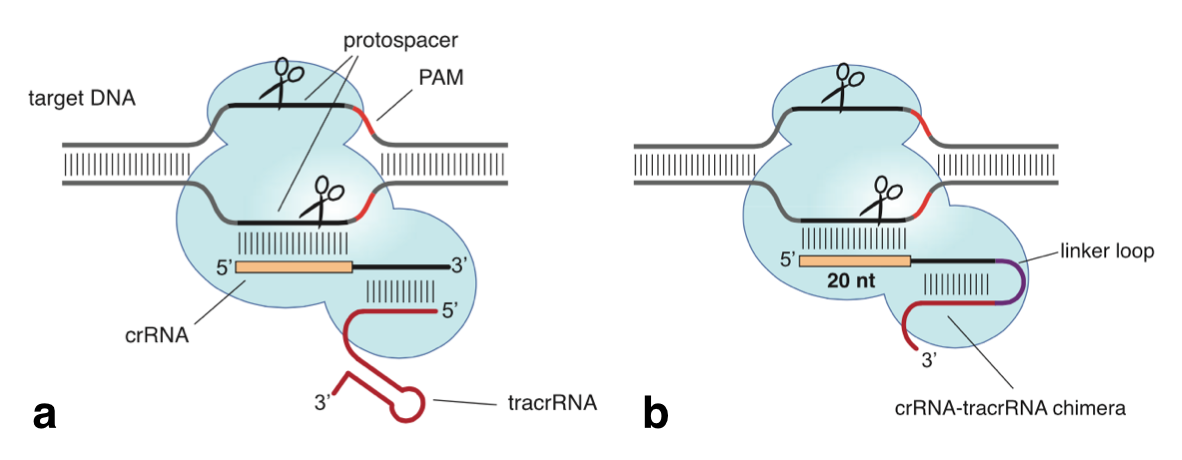
\includegraphics[width=1.15\textwidth]{figures/grna.png}
	}
	\caption{An RNA complex guides Cas9 to its target. \textbf{(a)} The matured crRNA and tracrRNA complex to guide Cas9. \textbf{(b)} A single gRNA comprising of the crRNA, a linker loop, and a crRNA guides Cas9 with the same efficiency as the dual-guide system. (Adapted from Jinek and Chylinski \textit{et al.} 2012)}
	\label{fig:grna}
	\end{center}
\end{figure}

Finally, realizing that the CRISPR-Cas system could be an easily programmable nuclease, the authors constructed a synthetic platform that marked the first time that this system was engineered for easier biotechnological use. They fused the tracrRNA and crRNA sequences (as they would be after maturation by RNAseIII) together with a short linker loop and expressed the entire construct as a single sequence. This led to high cleavage activity, indicating that bypassing the maturation step increases the activity of CRISPR-Cas restriction. This fused RNA molecule concept, dubbed the guide RNA (gRNA) is now nearly universally used in all applications of the CRISPR-Cas platform.

Perhaps one of the largest questions in the CRISPR-Cas9 field is that of targetability. Since there is a PAM sequence requirement for all known Cas9 proteins, each can only target a limited subset of all possible genomic targets. Interestingly, since the CRISPR-Cas system evolved as a bacterial immune system against viral DNA, and since different bacterial strains are attacked by vastly different phages, Cas9 proteins from different strains seem to have differing PAM specificities. Thus, the targeting range of the CRISPR-Cas platform can be expanded by adding more Cas9s to choose from (Kleinstiver \textit{et al.} 2015). We explore this further in chapter 5. Additionally, we explore the ability of Cas9 to distinguish between a match and a mismatch between the spacer and target at each position through a spacer randomization assay, which is described in chapter 6.

Of similar import is specificity. Because RNA and DNA can form complementary complexes even in the presence of a small number of mismatches between the two molecules' sequences, CRISPR-Cas9 often cleaves at off-target locations in a somewhat unpredictable manner. This has huge implications in applications of CRISPR-Cas9, as off-target mutagenesis can possibly have catastrophic effects on a cell. We have recently described an assay for detecting off-target cleavage events by Cas9 in an unbiased manner, which can be used to better understand the specificities of different Cas9 proteins (Tsai \textit{et al.} 2015). We explore the preliminary results of the application of the GUIDE-seq assay in chapters 3 and 4.

% Background section
\chapter{Background}
\label{Background}

Much of the recent history of genome editing consists of building the site-specificity of a nuclease through engineered protein-DNA interactions. Though this technique has proven effective and useful, as seen in the examples of Zinc-Finger Nucleases (ZFNs) and Transcription Activator-Like Effector Nucleases (TALENs), these platforms are difficult to use because of the complexity of programming protein-DNA specificity. In recent years, the CRISPR-Cas bacterial immune system has been extensively used as a genome engineering alternative that relies on RNA-DNA complementarity as the homing interaction that guides the specificity of the Cas9 nuclease. The ease of using such a platform to cleave specific sites in the genome simply by choosing a guide RNA sequence complementary to the target sequence has lead to an explosion in its use, with enormous amounts of interest and capital being contributed to the investigation of further development and application of this technology (Doudna and Charpentier \textit{et al.} 2014).\\

The molecular basis of Cas9 specificity comes from two independent RNA sequences: the CRISPR RNA (crRNA) and the transactivating CRISPR RNA (tracrRNA). In the wild, the tracrRNA and crRNA complex at a region of complementarity, are processed by endogenous nonspecific exonucleases, and then associate with Cas9 for a final crRNA-tracrRNA-Cas9 complex. When using the system in the lab, the crRNA and the tracrRNA are expressed as a single guide RNA (gRNA) strand to simply the formation of the final RNA-Protein complex. Cas9 then scans genomic DNA for a short Protospacer-Adjacent Motif (PAM) sequence, which is hard-coded into the protein. Once a match is found, Cas9 then alters its conformation to check for complementarity between the 20 nucleotide gRNA spacer sequence and the adjacent genomic DNA. If a match is found, Cas9 then makes a double stranded break at that locus (Jinek \textit{et al.} 2012, Anders \textit{et al.} 2014).

Once a double stranded break occurs in a eukaryotic cell, cellular machinery quickly repairs the break through either non-homologous end joining (NHEJ) or homology directed repair (HDR). In the case of NHEJ, random blunt end resections or small nucleotide insertions can occur, causing a deletion or insertion of one or more nucleotides in the final repaired site. This is phenomenon is often used to induce frame-shift mutations into a gene to  knock it out. In the case of HDR, a donor strand of DNA is used to template a precise insertion at the site of repair (Doudna and Charpentier 2014).

Perhaps one of the largest questions in the CRISPR-Cas9 field is that of targetability. Since there is a PAM sequence requirement for all known Cas9 proteins, each can only target a limited subset of all possible genomic targets. Interestingly, since the CRISPR-Cas system evolved as a bacterial immune system against viral DNA, and since different bacterial strains are attacked by vastly different phages, the Cas9 proteins from different strains seem to have differing PAM specificities. Thus, the targeting range of the CRISPR-Cas platform can be expanded by adding more Cas9s to choose from (Kleinstiver \textit{et al.} 2015).

Of similar import is specificity. Because RNA and DNA can form complementary complexes even in the presence of a small number of mismatches between the two molecules' sequences, CRISPR-Cas9 often cleaves at off-target locations in a generally unpredictable manner. This has huge implications in applications of CRISPR-Cas9, as off-target activity can possibly have catastrophic effects on a cell. We have recently described an assay for detecting off-target cleavage events by Cas9 in an unbiased manner, which can be used to better understand the specificities of different Cas9 proteins (Tsai \textit{et al.} 2015).


\newpage

\section{Selected Cas9 Proteins}

\begin{table}[h!]
\centering
\label{my-label}
\begin{tabular}{|l|l|l|}
\hline
{\bf Strain}                                        & {\bf CRISPR System Type} & {\bf Putative PAM} \\ \hline
{\it Lactobacillus buchneri}                   & Type II-A                & 5'-AAAA-3'         \\ \hline
{\it Neisseria meningitidis}                & Type II-A                & 5'-NNNNGATT-3'     \\ \hline
{\it Francisella novicida}                     & Type II-B                & 5'-NG'3'           \\ \hline
{\it Campylobacter jejuni}                          & Type II-C                & 5'-NNNNACA-3'      \\ \hline
{\it Pasteurella multocida} & Type II-C                & 5'-GNNNCNNA-3'     \\ \hline
\end{tabular}
\caption{Selected Cas9 proteins and their strains of origins and putative (predicted) PAM sequences.}
\end{table}

The five orthogonal Cas9 proteins selected for characterization are from a variety of families and CRISPR system subtypes, and have very disparate putative PAM sequences. All orthologs were chosen from the phylogenetic tree of Cas9 orthologues presented in the supplemental documents in  Fonfara \textit{et al} (2013). Note the inclusion of \textit{N. meningitidis} Cas9, which has been profiled previously in the literature, and will be used in part as a positive control. It should also be noted that all selected Cas9s have been shown to have \textit{in vitro} activity with a dual-RNA (non-chimeric) guide in the supplemental information of Fonfara \textit{et al} (2013).


\section{Experimental Approach}

\subsection{Prediction of RNA Guides}
The first step in using any Cas9 is to determine its crRNA and tracrRNA to construct a chimeric gRNA to guide the Cas9 activity. In general (for type II CRISPR systems), the Cas9 open reading frame, CRISPR repeats, and tracrRNA are all very near one another, generally within a single $\approx 5kb$ stretch. The location of these loci can easily be found through a simple BLAST search of SpCas9 against the bacterial genome to find the orthogonal Cas9 gene. Then, a repeat masking algorithm is applied to find fixed-length repeats in the region $\pm 2kb$ from the Cas9 protein. These repeats are the CRISPR repeats, which are spaced by fixed-length spacer sequences. Finally, the crRNA repeats are aligned against the same $\pm 2kb$ region to find the tracrRNA, which starts at the region of complementarity and ends at a poly-T transcriptional termination signal. Once these two sequences are found, they are fused together via a GAAA linker loop to form a single gRNA. This method was used computationally implemented to predict (with success) the gRNA for SaCas9 in Kleinstiver \textit{et al.} 2015. The same pipeline will be used to predict the crRNA, tracrRNA, and gRNA of the orthogonal Cas9 proteins in this study.



\subsection{Positive Selection}

To test if the predicted gRNA can indeed transactivate and guide the orthogonal Cas9 protein, a positive selection assay will be used. In this assay, a toxic gene is placed in front of a glucose-inducible promoter on a plasmid containing a set Cas9 target site containing the predicted PAM sequence. The plasmid is co-transformed with a plasmid containing both the orthogonal Cas9 gene and the gRNA gene and the bacteria are grown in glucose-containing media. If there is bacterial growth, then the gRNA activated and guided Cas9 to cleave the target site on the toxic plasmid-containing gene, keeping the bacterium alive. Thus, this positive selection experiment can be used as an early screen for gRNA efficiency.

\subsection{Negative PAM Depletion Assay}

Once the gRNA is confirmed to work through the positive selection assay, a negative selection assay will be used to fully characterize the PAM specificity of the protein. In this assay, an antibiotic resistance gene is placed on the same plasmid as a fixed target site followed by a randomized 8bp PAM region (i.e. NNNNNNNN). This plasmid is co-transformed with a plasmid containing the orthogonal Cas9 and gRNA, and the bacteria are grown in antibiotic-containing media. If the randomized PAM matches the Cas9 PAM, then the resistance plasmid is cleaved, and the bacterium dies. At the end of the assay, the region containing the spacer and PAM is sequenced using high-throughput sequencing. The relative abundance of each PAM sequence is analyzed computationally. PAM sequences that are the most depleted are the most active PAM sequences for the Cas9 protein. An example of the results from this assay, as found in Kleinstiver \textit{et al.} 2015 can be found in Figure 1. The code used to determine relative PAM frequencies can be found in the supplemental information of that same text.

\begin{figure}
\begin{center}
\begin{tabular}{ | l | l | l | }
\hline
	\textbf{PAM} & \textbf{Count} & \textbf{Frequency} \\ \hline
	GTT & 27360 & 3.00391958805898E-2 \\ \hline
	TGT & 26445 & 2.9034595579758699E-2 \\ \hline
	TTT & 24614 & 2.70242970542704E-2 \\ \hline
	GGT & 23149 & 2.5415838649114501E-2 \\ \hline
	TAT & 22106 & 2.42707040985496E-2 \\ \hline
	TGC & 21063 & 2.3125569547984798E-2 \\ \hline
	AGT & 20840 & 2.2880732534776699E-2 \\ \hline
	GCT & 20368 & 2.2362512488883501E-2 \\ \hline
	\vdots & \vdots & \vdots \\ \hline
	TAG & 6433 & 7.0629439729471598E-3 \\ \hline
	CAG & 4531 & 4.9746928558096603E-3 \\ \hline
	AAG & 866 & 9.5080203335492597E-4 \\ \hline
	GAG & 457 & 5.0175118850254196E-4 \\ \hline
	GGG & 386 & 4.2379859685335002E-4 \\ \hline
	TGG & 322 & 3.5353147198647402E-4 \\ \hline
	AGG & 309 & 3.39258462247889E-4 \\ \hline
	CGG & 278 & 3.0522282364049599E-4 \\ \hline
\end{tabular}
\caption{Table Excerpt of PAM Depletion Assay analysis for EGFP site 1 for wild-type \textit{S. pyogenes} Cas9. Cells are in descending frequency order. Note that the most depleted PAM sequences are those in the format NGG, and are depleted by two orders of magnitude. The second most depleted set are those in the format NAG, which are less depleted but still somewhat depleted compared to the rest of the PAM sequences.}
\end{center}
\end{figure}

\newpage
\subsection{GUIDE-Seq Specificity Profiling}
GUIDE-Seq is a method for unbiased detection of off-target nuclease activity that we recently described in Tsai \textit{et al.} 2014. In this assay, a short, end-stabilized DNA strand is captured into double stranded breaks through NHEJ capture, wherein the blunt ends of the oligo is captured into the blunt double stranded break by endogenous DNA repair machinery. These regions are then linearly amplified off of the known oligo sequence and sequenced with high-throughput sequencing. By mapping these sequences back to the genome, the sites of off-target cleavage events are elucidated.

In this study, GUIDE-seq will be performed for each orthogonal Cas9 for a number of targetsites to determine the number of off-target cleavage events that each protein is generally responsible for. This will provide a set of data that will be valuable in determining which Cas9 is best used in a given application (e.g. a Cas9 with very low off-target effects may be better for therapeutic applications).

\subsection{Expected Results and Potential Roadblocks}

The methods outlined above are, in a way, a ``Hail Mary" approach to test the activity of the selected Cas9s. For the positive selection to work, three things must simultaneously be successful. First, both the chimeric guide and the Cas9 must both be successfully expressed in high numbers, and be non-toxic to the cell. Second, the predicted crRNA and tracrRNAs must be correct, and the chimeric guide constructed from them must activate and guide the Cas9. Third, the Cas9 must induce a double stranded break in the targeted DNA sequence. Only then will the plasmid containing the toxic gene be degraded, and the cell will live. To ensure that the system should work in its totality, the \textit{N. meningitidis} Cas9 (NmCas9) will be used as a positive control, as it has been profiled in a number of published studies, and so its activity in the positive selection can be expected. In the case of further complications, individual steps of the expression and cleavage process will be evaluated. For example, the expression of the protein and the gRNA could be evaluated via RT-qPCR. One other possible concern is whether or not the tracrRNA secondary structure in the gRNA will accurately reflect the endogenously processed tracrRNA that would ordinarily transactivate the Cas9 protein. For this reason, multiple different truncations of the tracrRNA will be predicted and tested. Though we expect at least some nonempty subset of the 5 selected Cas9s to work in this assay, it is possible that only the NmCas9 will work successfully, and that the other four Cas9s simply do not work \textit{in vivo} outside of their host organisms.

The negative PAM depletion assay also carries a few assumptions that must be taken into consideration. In particular, the random 8bp PAM is assumed to be fully random, with every sequence having an equal probability of appearing. However, due to inherent biases in the oligonucleotide synthesis process, this is not always indeed the case. To account for this, the PAM depletion assay will be carried out with the same randomized PAM library with \textit{S. pyogenes} Cas9, which has the most well-characterized PAM sequence. In doing so, we can make sure that there are not significant biases in the PAM library that may skew our PAM characterization results.

If we show that one or more of these Cas9s have activity \textit{in vivo}, then the overall sequence specificity of the Cas9 can be profiled in an unbiased fashion through GUIDE-Seq. Though we have shown previously that off-target profiling cannot be theoretically or computationally predicted (Tsai \textit{et al.} 2015), we hypothesize that Cas9s with shorter putative PAM sequences (e.g. \textit{F. novicida}, which has a putative PAM of 5'-NG-3') will have less stringent sequence specificity.

\chapter{GUIDE-Seq: An unbiased assay for genome-wide off-target detection}
\section{Exploratory Analysis of Potential Off-Target sites}
\section{Overview of the GUIDE-Seq Assay for Production of Raw Read Data}
\section{Bioinformatic Analysis of GUIDE-Seq data to infer off-target sites}
\section{Comparison of GUIDE-Seq results to ChIP-Seq and Computationa}

\chapter{\textit{guideseq}: A computational pipeline for analyzing GUIDE-Seq data}
\section{Understanding the core steps of the \textit{guideseq} pipeline}
\section{Example output of the software}

\chapter{Expanding the Targeting Range of CRISPR-Cas with Orthogonality Profiling and Protein Engineering}
\section{Engineering the PAM-contacting residues of Cas9}
\section{Predicting the Activity of Orthogonal Cas9 Systems}
\section{Understanding the PAM Depletion Assay}
\section{PAM Depletion Assay Results}

\chapter{Characterizing the Specificity of CRISPR-Cas Proteins}
\section{Overview of the spacer subsequence randomization assay}
\section{Specificity Results of Randomization Assay}

\chapter{CasBLASTR: A tool for Genome Editing Experiment Design and Analysis}
\section{Application Architecture}
\section{Results and Usage Statistics}

\chapter{Conclusion and Future Steps}

%\chapter{Introduction}
\label{introduction}

Much of the recent history of genome editing consists of building the site-specificity of a nuclease through engineered protein-DNA interactions. Though this technique has proven effective and useful, as seen in the examples of Zinc-Finger Nucleases (ZFNs) and Transcription Activator-Like Effector Nucleases (TALENs), these platforms are difficult to use because of the complexity of programming protein-DNA specificity.
In recent years, the CRISPR-Cas bacterial immune system has been extensively used as a genome engineering alternative that relies on RNA-DNA complementarity as the homing interaction that guides the specificity of the Cas9 nuclease. The ease of using such a platform to cleave specific sites in the genome simply by choosing a guide RNA sequence complementary to the target sequence has lead to an explosion in its use, with enormous amounts of interest and capital being contributed to the investigation of further development and application of this technology (Doudna and Charpentier \textit{et al.} 2014).
%
%The molecular basis of Cas9 specificity comes from two independent RNA sequences: the CRISPR RNA (crRNA) and the transactivating CRISPR RNA (tracrRNA). In the wild, the tracrRNA and crRNA complex at a region of complementarity, are processed by endogenous nonspecific exonucleases, and then associate with Cas9 for a final crRNA-tracrRNA-Cas9 complex. When using the system in the lab, the crRNA and the tracrRNA are expressed as a single guide RNA (gRNA) strand to simply the formation of the final RNA-Protein complex. Cas9 then scans genomic DNA for a short Protospacer-Adjacent Motif (PAM) sequence, which is hard-coded into the protein. Once a match is found, Cas9 then alters its conformation to check for complementarity between the 20 nucleotide gRNA spacer sequence and the adjacent genomic DNA. If a match is found, Cas9 then makes a double stranded break at that locus (Jinek \textit{et al.} 2012, Anders \textit{et al.} 2014).
%
%Once a double stranded break occurs in a eukaryotic cell, cellular machinery quickly repairs the break through either non-homologous end joining (NHEJ) or homology directed repair (HDR). In the case of NHEJ, random blunt end resections or small nucleotide insertions can occur, causing a deletion or insertion of one or more nucleotides in the final repaired site. This is phenomenon is often used to induce frame-shift mutations into a gene to  knock it out. In the case of HDR, a donor strand of DNA is used to template a precise insertion at the site of repair (Doudna and Charpentier 2014).
%
%Perhaps one of the largest questions in the CRISPR-Cas9 field is that of targetability. Since there is a PAM sequence requirement for all known Cas9 proteins, each can only target a limited subset of all possible genomic targets. Interestingly, since the CRISPR-Cas system evolved as a bacterial immune system against viral DNA, and since different bacterial strains are attacked by vastly different phages, the Cas9 proteins from different strains seem to have differing PAM specificities. Thus, the targeting range of the CRISPR-Cas platform can be expanded by adding more Cas9s to choose from (Kleinstiver \textit{et al.} 2015).
%
%Of similar import is specificity. Because RNA and DNA can form complementary complexes even in the presence of a small number of mismatches between the two molecules' sequences, CRISPR-Cas9 often cleaves at off-target locations in a generally unpredictable manner. This has huge implications in applications of CRISPR-Cas9, as off-target activity can possibly have catastrophic effects on a cell. We have recently described an assay for detecting off-target cleavage events by Cas9 in an unbiased manner, which can be used to better understand the specificities of different Cas9 proteins (Tsai \textit{et al.} 2015).
%\begin{savequote}[75mm]
Don't get fooled by people who claim to have a solution to Artificial General Intelligence... Ask them what error rate they get on MNIST or ImageNet.
\qauthor{Yann LeCun}
\end{savequote}


\chapter{The Luna Rating System}

\section{Introduction}

On March 12, 2016, just after 5 pm in Seoul, Lee Se-dol, the 18-time world champion of the board game Go, conceded defeat. His opponent had trounced him in three consecutive games, stunning him with unexpected moves and overwhelming him with a demonstrated mastery of the game's finest details. The man who placed the winning stones onto the Go board swiftly stepped aside to reveal the series' true victor: an Artificial Intelligence (AI) developed by Google DeepMind called AlphaGo\cite{silver2016mastering}. The outcome was heralded internationally as a revolutionary achievement for AI. ``AlphaGo's victory means the world is about to change,'' proclaimed \textit{The Next Web}\cite{1_nextweb_2016}. ``Artificial intelligence [has come] of age in showdown between human brainpower and a machine,'' \textit{the Guardian} similarly declared\cite{1_the_guardian_2016}. 

To long-time observers of AI research, these headlines likely look familiar. The sensation is similar to the coverage of Eugene Goostman's so-called passing of the Turing Test --- ``a milestone in artificial intelligence,'' said \textit{the Guardian}\cite{1_the_guardian_2014, occasional_pamphlet_2014} --- and the wave of hype surrounding Watson's victory in Jeopardy! --- ``a vindication for the academic field of artificial intelligence,'' reported \textit{The New York Times}\cite{1_newyorktimes_2011}. In these cases and others, after the dust settles, the significance of the achievement in the context of general AI research remains unclear. Expert views on the current state of AI could not be more varied or discordant. One representation of this disarray is the recent collection of essays on \textit{What to Think About Machines that Think}, in which over 200 leading thinkers disagree on the definition, timeline, and even theoretical possibility of AI \cite{edge2016what}. There is no shortage of speculation, nor any sign of consensus, on the emergence of truly intelligent machines.

Day-to-day research in artificial intelligence proceeds unencumbered by these speculations. A model's worth is not measured by public perception, but rather, according to its performance on benchmarks of the field. Such benchmarks --- e.g. object recognition in ImageNet \cite{russakovsky2015imagenet}, language modeling in the 1 Billion Word Dataset \cite{chelba2013one}, reinforcement learning for various Atari Games\cite{mnih2013playing} --- are attractive for researchers who are seeking measurable, specific improvements on the state of a particular art. As guiding lights for research efforts, these benchmarks can have tremendous influence on AI. In the best case, they can provide cohesion and order to a burgeoning field. Unfortunately, they can also incentivize incremental progress on narrow problems and effectively discourage large leaps of innovation\cite{shieber2015}. Moreover, these benchmarks give researchers little insight as to a model's proximity to true AI. Apparent progress on a particular task --- object recognition, chess, Go, etc. --- may actually be negligible in the long arc of AI research.

In this thesis, I present an original benchmark for true AI, arguably the first of its kind. The benchmark, which I call Luna\footnote{Luna is an tribute to Alan Turing; Luna Rating is an anagram of Alan Turing.}, takes inspiration from the network-based rating systems of chess and the natural language interrogations of the Turing Test. Luna invites humans and machines to participate in two-player games in which each player assesses the intelligence of the other. The aggregation of these assessments is used to assign a rating to the player. In this sense, the ratings that emerge from the system are the results of a never-ending test of each of the player's general AI. The definition of intelligence is not presupposed in this system; instead, it emerges from the collective judgement of all players. Thus the system is a microcosm of the natural process that humans use to evaluate each other's intelligences. I will argue that the system offers a bright guiding light on the dim path towards machine intelligence.

\section{Existing Tests for AI}

The history of testing AI is long but sparse. It begins in 1950 with the introduction of the Turing Test and meanders into the present day with a focus on specialized tasks. Only recently has there been interest in designing new tests that are more appropriate for practically evaluating general AI \cite{you2015beyond}. This interest often manifests as an appeal to move ``beyond the Turing Test'' \cite{1_the_newyorker_2015}. However, the Turing Test has never been a practical test for general AI. Thus the recent wave of interest is really a call for the first ever practical test for general AI.

\subsection{The Turing Test}

The first formal test for machine intelligence was articulated by Alan Turing, the father of computer science and one of the progenitors of AI \cite{turing1950computing}. Six decades later, the eponymous Turing Test remains at the center of the dialogue surrounding machine intelligence. The Test requires three rooms, each equipped with a telegraph. In one room, the machine candidate for AI is connected to the telegraph, ready to receive and transmit messages. The second room, which is disconnected from the first room, houses a human confederate. A human judge resides in the third room with telegraph connections to the first and second room. The duty of the judge is to determine which room contains the human. Different instantiations of the Test vary details beyond this framework, e.g. how long the conversations go on before a judgment is made \cite{loebner2003home, bishop2010testing}. In all cases, the machine is deemed intelligent if it is able to trick the human judge into guessing that it is human.

Since its proposal, the Turing Test has weathered criticism from every conceivable angle. There are myriad philosophical objections, especially those of Block, Gunderson, and Searle, who argue that intelligence is by definition a capacity, and that the Test cannot prove the existence of capacity  \cite{block1980intuitions, gunderson1964vii, searle1980minds}. Shieber saves the Test from this line of critique using Interactive Proofs as a metaphor \cite{shieber2007turing}, but maintains that the Test should be viewed as a thought experiment, rather than a practical inducement for research \cite{shieber2015}. Hayes \& Ford agree with the impracticality of the Test \cite{hayes1995turing}. They go so far as to call the Test ``harmful'' for AI research, citing the lack of restrictions placed on judges, the emphasis on deception, and the binary result as fundamental failures of the Test. Indeed, attempts at practical instantiations of the Test (e.g. the Loebner Prize) have been met with strong criticism from the research community \cite{shieber1994lessons, occasional_pamphlet_2014}. The Test remains synonymous with AI in the public parlance, but researchers are increasingly looking ``beyond the Turing Test'' for more practical tests of AI \cite{1_the_newyorker_2015, you2015beyond}.

\subsection{Robotics Contests}

Robotics seems like a natural domain for testing artificial intelligence. The prospect of robots that are able to behave and reason at human levels is a clear motivation for AI research. Moreover, a candidate for AI is likely to be more convincing if it is physically instantiated. Anderson, Baltes, and Cheng (2011) review existing robotics contests and critique their utilities as benchmarks for AI research. These contests include annual competitions like AAAI/IJCAI, which consists of a diverse suite of tasks for the robots to perform \cite{balch2002ten}; RoboCup, which requires candidates to play an actual game of soccer, thus entering the realm of multi-agent strategizing \cite{kitano1997robocup}; and HuroCup, which might be considered an ``olympics for robots'', requiring contestants to compete in a wide range of sports and agility competitions \cite{baltes2009hurocup}. Anderson, Baltes, and Cheng find specific shortcomings in each of these competitions as proxies for AI, but suggest that more broad and versatile robotics competitions could still be useful for testing AI.

I argue that a test for AI should be independent of robotics. One inherent problem with robotics as a medium to test AI is that there are a host of extremely challenging problems in the field that have little or nothing to do with intelligence (e.g. the difficult mechanical problems associated with walking). It may be that certain problems in robotics are sufficient to demonstrate AI, but those problems are often harder than AI itself. Another fundamental problem in robotics competitions that currently exist is that they consist of a fixed set of a tasks. Any fixed set of tasks is susceptible to be criticized by third parties as unrepresentative of AI. Moreover, a robot can be trained to accomplish this fixed set of tasks without possessing any unifying architecture for general AI. Thus, robotics should be seen not as a medium for testing AI, but rather as an application of AI once it has been reached. Too keen of a focus on robotics threatens to pull research away from the most direct path towards AI. 

\subsection{Specialized Benchmarks}

The overwhelming majority of testing in modern AI research is performed on specialized benchmarks. ImageNet, which requires contestants to recognize objects in a massive image dataset, is a well known example \cite{russakovsky2015imagenet}. Various Natural Language Processing problems, such as Part of Speech Tagging and Language Modeling, are often studied using the Penn Treebank dataset as a benchmark \cite{marcus1993building}. Mnih et al. establish a suite of Atari games as a benchmark for reinforcement learning \cite{mnih2013playing}. Several contests focus on AI game playing, such as chess \cite{hayes1976world}, poker \cite{littman20062006}, and general game playing \cite{genesereth2005general}. The Hutter Prize offers a benchmark for lossless text compression \cite{mahoney2006rationale}. None of these competitions claim to test general AI. The search for a practical test for AI continues. 

\section{A Pragmatic Sufficiency for Intelligence}

Given the substantial and sustained research attention that AI has enjoyed, the lack of a unified practical benchmark may be rather surprising. This absence can be partly explained by the lack of consensus surrounding the definition of intelligence. Psychology and AI suggest several definitions of the term. Legg and Hutter collect 70 distinct definitions from both fields, admitting that even this list is incomplete \cite{legg2007collection}. To further complicate matters, intelligence is also entangled with other philosophical quandaries, such as the nature of consciousness. The Turing Test sidesteps the definition problem by suggesting a sufficient condition without claiming that the condition is also necessary; passing the Test is enough to demonstrate intelligence, but failing does not prove its absence. However, as alluded to above, even this sufficient condition is vulnerable to philosophical criticism. It seems as though any proposed definition or sufficiency for intelligence will invariably be contested.

In search of a path around this philosophical obstacle, I begin with a tautological observation: a machine would be called intelligent if everyone called it intelligent. If the machine simply generated random sequences of letters and was able to ``feign intelligence'' by random luck, it would still be called intelligent. (In the same way, a human randomly guessing on an IQ test could be deemed intelligent by chance, or a non-Italian speaker visiting Italy could feign fluency by randomly blurting out syllables and getting lucky.) Such a randomly lucky machine would be evidence of weak AI, but not of strong AI, to use the terminology of Searle; weak AI requires only the apparent simulation of a mind, while strong AI insists that a machine \textit{is} a mind \cite{searle1980minds}. For the purpose of developing a practical test, measuring weak AI suffices. Russell and Norvig, authors of the most widely cited textbook on AI, confirm this view, remarking that ``most AI researchers take the weak AI hypothesis for granted, and don't care about the strong AI hypothesis'' \cite{russell1995modern}. If a machine is able to convincingly demonstrate intelligence to everyone in the world, surely that would be sufficient to call it weak AI.

Of course, the requirement that everyone weigh in on the intelligence status of a machine is impractical and overly strict. At the same time, a benchmark relying on human judgements must be sufficiently standardized so that subjective variations do not prevent meaningful comparisons between test instances. And yet standardization threatens to impose an implicit definition of intelligence. To resolve this paradox, I take inspiration from the rating systems of chess \cite{glickman1995chess}. The rating assigned to a chess player is meant to reflect that player's ability relative to all other rated players. These ratings are not assigned based on complete tournaments in which every player challenges every other player; rather, the ratings are awarded based on the individual outcomes of two-player games. Each game is seen as a sample of the player's ability, and ratings are updated after each game to take into account this new sample. Thus the ratings are constantly moving towards true representations of the relative abilities of all players. Chess rating systems are able to assign a rating to a player that reflects the consensus of all players in the system, without relying on every player for every rating.

With chess rating systems and the Turing Test in mind, I propose the following pragmatic sufficiency for AI: \textbf{if human consensus deems the verbal responses of a machine to be evident of intelligence comparable with that of most other humans, then the machine is intelligent.}  Of course, this sufficiency as stated leaves many questions unanswered. How many humans must directly provide input in order to capture consensus? What precisely is meant by ``comparable'' and ``most''? These are questions that may be addressed philosophically or empirically. But for the purpose of developing a benchmark, it suffices to measure relative progress: if human consensus deems the verbal responses of one machine to be more evident of intelligence than those of another machine, then the former is closer to achieving AI. Similarly, as the number of humans providing direct inputs increases, accuracy increases, as the collective judgement will converge towards the consensus. This pragmatic sufficiency for intelligence forms the foundation of the Luna Rating System, my proposed benchmark for AI.

\section{The Luna Rating System}

\subsection{The Luna Rating System}

The Luna Rating System (LRS) is a never-ending tournament of a two-player game called the Luna Game. The details of the Luna Game are covered in Chapter 2. For the purpose of introducing LRS, it suffices to say that a Luna Game requires each of the two players to guess the intelligence, or Smarts Rating, of the other player. The winner of the game is the player whose guess is closest to the actual rating. At the end of a Luna Game, a player's Smarts Rating is updated based on the opponent's guess. Players are encouraged to maximize their own Smarts Ratings and their number of game wins. They are therefore incentivized to demonstrate maximal intelligence and to judge the intelligence of other players with maximal accuracy. The symmetry of the Luna Game is intentional: every player in LRS is constantly a judge of intelligence and a candidate under evaluation by other players.

In benchmarking AI, the central quantity of interest in LRS is a player's Smarts Rating. This number encapsulates the human consensus of the intelligence of that player. If a machine achieves a Smarts Rating that is on par with the Smarts Ratings of humans, after a sufficient number of Luna Games, it will have passed the implicit intelligence test of LRS and convincingly demonstrated general AI. Moreover, the effect of changes made to the machine may be measured according to the subsequent difference in Smarts Rating. The Smarts Rating is the number that should be reported in characterizing the success of a candidate for AI.

One immediate advantage of LRS is its strong incentive for judges to perform their duties well. No other testing system for AI with human judges has a built-in impetus for high quality judging. Moreover, as the details of the Luna Game make clear, judges are not perversely motivated to attempt to fool candidates for AI by putting forth excessively difficult tests; instead, they are rewarded for giving judgments that are close to the consensus of all players in the system. Another critical advantage of LRS is the continuity of Smarts Ratings. As opposed to binary systems like the Turing Test, progress, however small, is observable. This property distinguishes LRS as an informative benchmark, rather than a theoretical test. An additional feature of LRS is its accessibility. The system is meant to be freely and constantly available to researchers, e.g. through the World Wide Web. These characteristics and others significantly differentiate LRS from existing tests for AI. Moreover, as I argue in the following section, LRS is unique in satisfying all of the fundamental principles of a practical test for intelligence.

\subsection{Principles of a Practical Test for Intelligence}

LRS is meant to steer AI research towards the creation of general intelligence. Therefore, the system must actually be used; a thought experiment will not suffice. Here I propose five principles that must be obliged if the test for intelligence is to fulfill its stated purpose.

\subsubsection{Accessibility}
To serve as a useful guide, the test for AI must be constantly accessible to researchers. Ideally the test should be efficient enough that it may be used several times throughout the course of an AI developer's day. This principle discourages a centralized competition that is only held at regular intervals, and instead favors a rating system that can be accessed through the Internet and then carried out using the resources of an average computer.

\subsubsection{Generalizability}
A test need not span all possible areas of intelligence, but the results should reflect the subject's ability to perform in all areas. In this sense, the test should be \textit{AI-complete} --- a machine that does well on this test should do similarly well on any other reasonable test of intelligence. The proposition of the Turing Test, which continues to be held by many researchers, is that the problem domain of natural language is AI-complete. The system proposed here shares this premise.

\subsubsection{Continuity}
Every candidate for AI should be able to observe changes in performance over the course of development. A test that only reports a binary outcome --- pass or fail --- will not be useful for researchers who are not yet close to passing. The test's outcome should instead be continuous, indicating clearly when progress is being made.

\subsubsection{Dependent on People, Independent of Persons}
A fair test should not rely on any one person's interpretation of intelligence. At the same time, intelligence is a social construct that cannot be reasonably appraised without input from humans. Therefore a test for intelligence must take into account the popular conception of intelligence, but it cannot rely on any single human judge to determine its outcome.

\subsubsection{Immunity to Gaming}
It should not be possible for a researcher to ``game the system'' and achieve outsized results by exploiting structure in the test. This principle precludes any sort of hard-coding of knowledge that is \textit{a priori} known to be important for the test. For example, a standardized test fails the Immunity to Gaming principle, since any researcher who observes the results of the test once would be able to submit a machine with the memorized knowledge necessary to pass the test. 

\subsection{Analysis of Principles}

LRS is the only practical test for intelligence to satisfy all five of the principles outlined above. The system exists online and invites humans and machines to play for free. Thus LRS is maximally accessible. Like the Turing Test, the Luna Game involves open-domain question answering, and therefore is AI-complete, i.e. generalizable to all problems in AI. Smarts Ratings are continuous quantities that are updated after every Luna Game, making progress immediately clear to all players. These ratings reflect the equilibrium consensus of all players in LRS on what it means to be intelligence, and is not biased towards any single player's notion. Finally, the system is immune to gaming, since all players are encouraged to devise their own original questions, which cannot be predicted by the other player. Table \ref{principles} summarizes how the satisfaction of these five principals represents a substantial improvement over existing tests for AI.

\begin{table}[h!]
\centering
\begin{tabular}{|l|l|l|l|l|l|l|}
\hline
\textbf{Principle}                                                                              & \textbf{Turing} & \textbf{ImageNet} & \textbf{HuroCup} & \textbf{Hutter} & \textbf{Games} & \textbf{LRS} \\ \hline
Accessibility                                                                          &        & \checkmark        &         & \checkmark      & \checkmark     & \checkmark   \\ \hline
Generalizibility                                                                       & \checkmark      &          & \checkmark       &        &       & \checkmark   \\ \hline
Continuity                                                                             &        & \checkmark        & \checkmark       & \checkmark      & \checkmark     & \checkmark   \\ \hline
\begin{tabular}[c]{@{}l@{}}Dependent on People, \\ Independent of Persons\end{tabular} &        &          &         &        &       & \checkmark   \\ \hline
Immunity to Gaming                                                                     & \checkmark      &          &         &        & \checkmark     & \checkmark   \\ \hline
\end{tabular}
\caption{\label{principles}\textbf{The Luna Rating System is the only test that satisfies all five principles for a practical test of intelligence.} Other existing tests include the Turing Test, which invokes natural language; ImageNet, which focuses on object recognition in computer vision; HuroCup, a sports-based competition in robotics; the Hutter Prize, which deals with text compression; and several games, such as chess, poker, and general game playing.}
\end{table}

\subsection{Contrary Views on the Main Question}

In Turing's seminal paper introducing his Test, he includes a section titled ``Contrary Views on the Main Question,'' in which he enumerates and responds to anticipated objections \cite{turing1950computing}. Here I follow his lead, briefly considering possible objections to the Luna Rating System.

\subsubsection{Test Time Objection}

Given the reliance on human input, some may object that the time required to obtain meaningful results from LRS is too long. In practice, with a sufficient number of active participants, it should be possible to solicit tens of judgements per day. This timescale is actually far shorter than possible alternatives, especially when those alternatives require humans convening and thus may only occur once every several months or years. Even specialized tasks that do not require any human input can take several hours to return results. Of course, the test time may dramatically increase if human participation is lacking; this condition is addressed in the following objection.

\subsubsection{System Maintenance Objection}

Some may object that a system requiring such broad and consistent human participation is simply too expensive to maintain. In the case that the system is web-based, the standard technical difficulties associated with hosting a website must be addressed. Furthermore, participants must be recruited and persuaded to play. In Chapter 6, I present a proof-of-concept to address this objection, demonstrating that a web-based implementation of LRS can be launched and sustained with relatively limited cost. The success of this simple system suggests that a system with more explicit incentives, e.g. paying participants to play, would have no trouble sustaining the required levels of activity.

\subsubsection{Barrier to Entry Objection}

After reviewing the details of the Luna Game (presented in Chapter 2), some may object that the entry into LRS requires too much additional work on the part of AI researchers. I respond to this objection in Chapter 4 with a review of the extensive body of work on two longstanding AI problems: Question Generation and Question Answering. I demonstrate that entry into LRS requires negligible effort beyond addressing these two problems. Moreover, an approach to the relatively lesser known problem of Question Generation is actually optional; researchers may manually select a fixed set of questions without affecting the integrity of the test. Question Answering is an extremely active research area and LRS invites direct application of these efforts.

\subsubsection{Definition Drift Objection}

Some may object that Smarts Ratings might drift towards a specific notion that may or may not be related to intelligence. This could occur if players were primed with the suggestion to ask mathematical questions or trivia questions, for example. To prevent this drift, I insist that LRS provides minimal instructions to players as to what is meant by ``intelligence''. Beyond this lack of bias, the integrity of Smarts Ratings is contingent upon the assumption that players will behave according to their own intuitive notions of intelligence. The results presented in Chapter 6 corroborate the reasonableness of this assumption. Additional anecdotal evidence suggests that players enjoy the challenge of creating probing and diverse questions in the course of the game.

\subsection{Single Dimension Objection}

While Smarts Ratings are more expressive than binary outputs, some may object that a single dimension is insufficient to meaningfully capture intelligence. For example, the theory of multiple intelligences from psychology posits that intelligence is best described along eight or more axes\cite{gardner2011frames}. The proposed existence of the $g$ factor, a variable that has been shown to correlate with most other modules of intelligence, is one possible response to this objection \cite{visser2006g}. More generally, the conception of intelligence as a real value in a single dimension is motivated by the same practicality that underpins much of LRS; such a metric is the simplest way to capture progress or regress in the pursuit of AI.

\subsubsection{Malicious Strategizing Objection}

With a particular weariness of anonymous online players, some may object that malicious strategizing could threaten the integrity of the test. Indeed, if all players decide to behave randomly, the results output by LRS will not be meaningful. As discussed in Chapter 3, LRS does not rely on the honest intentions of all players, nor does it assume that players will always play to the best of their abilities. The one necessary assumption is that the majority of players will ``guess honestly''. The meaning of this requirement is revealed in Chapter 2, and the extent to which the system is vulnerable to malicious guessing is rigorously analyzed in Chapter 3.

\section{Thesis Outline}
The primary contribution of this thesis is the introduction of the Luna Rating System as a practical benchmark for machine intelligence. The remainder of the thesis is roughly divided into three parts. In the next chapter, I continue the introduction of LRS with a description of the Luna Game. This chapter is followed by a study of the robustness of LRS, characterizing likely strategies for game play and analyzing their effect on the accuracy of Smarts Ratings as a proxy for intelligence. Next I characterize the three subproblems that constitute the full Luna Game. The first two problems --- Question Generation and Question Answering --- have been extensively studied in previous work, which I review in Chapter 4. The third subproblem, which I deem the Luna Rating Prediction Problem, has not been previously characterized. In Chapter 5, I formalize the problem, argue its merit as a general problem of interest, and present baseline results. Finally, in Chapter 6, I create the first online instantiation of LRS and invite humans and machines to play. Their games illuminate the current state of AI and offer rich insight into the human conception of intelligence.

%\begin{savequote}[75mm]
But it is not conceivable that such a machine should produce different arrangements of words so as to give an appropriately meaningful answer to whatever is said in its presence, as the dullest of men can do.
\qauthor{Ren\'e Descartes}
\end{savequote}

\chapter{The Luna Game}

\section{Overview}

At the center of my proposed rating system is a two-player game that I call the Luna Game. Each player enters the game with a secret Smarts Rating, which has been assigned based on her performance in previous games. As the name suggests, the Smarts Rating is a proxy for the player's intelligence. The objective of the game is simple: guess the Smarts Rating of the other player. In other words, a player should strive to accurately evaluate the intelligence of her opponent. The winner of the Luna Game is the player whose guess is closest to the actual Smarts Rating of the other player. After the game, the opponent's guess is factored into the player's Smarts Rating so that the rating captures all the guesses of previous opponents.

As a player with a high Smarts Rating, why not ``play dumb''? This strategy would indeed induce an inaccurately low guess from the opponent, possibly leading to a win. However, the motives of a player reach beyond the scope of a single game. In addition to winning games, a player wants to achieve a high Smarts Rating. Since the rating depends on the guesses of all the player's opponents, she will need to ``play smart'' to accomplish her long term goal. The ``playing dumb'' method is not only detrimental to a player's rating, but also unsustainable as a consistent strategy; a player of that method will have her Smarts Rating lowered as a result, narrowing the margin between future opponents' guesses and her actual Smarts Rating if she continues to use the strategy. Players who remain and thrive will be those who play smart.

In designing the Luna Game, I sought to impose as few constraints as possible. The Game is meant to be a microcosm of the organic process for defining intelligence. Humans evaluate each other's intelligences through a series of questions and answers, often in the form of a written exam, but also informally through everyday conversations. The most natural notion of an individual's intelligence arises from the consensus of the people who perform these evaluations. A player's Smarts Rating is meant to reflect this natural notion; it is an aggregate of evaluations carried out by other players. To define the scope of an evaluation, I impose only those constraints necessary to motivate honest and repeated play.

A session of the Luna Game consists of three phases: the Interview Phase, the Response Phase, and the Guess Phase. During the Interview, each player creates a set of 5 questions to pose to the opponent. In the Response Phase, each player responds to the other's questions. Finally, in the Guess Phase, each player receives responses back from her opponent, and must use the responses to guess her opponent's Smarts Rating. I describe each of these phases in detail throughout the rest of this chapter and illustrate the game through examples of play.

\section{Interview Phase}

A Luna Game begins with the Interview Phase. During this phase, each player prepares a set of 5 free-form questions to be given to the other player. The number of questions represents a tradeoff between the time required to complete the phase and the difficulty of the guessing task. With more questions, each player would need more time to construct the questions, increasing the likelihood that they will quit the game and leave the system. With fewer questions, construction time could be shortened, but the informativeness of the subsequent responses would suffer, and the Smarts Ratings would ultimately be less meaningful. I chose the number 5 to optimize this tradeoff, but the number may be adjusted in future iterations of the system. In a similar practical vein, I insist that questions be constructed in batch, rather than allowing for sequential question-response. Since the game is played online, allowing for back and forth would increase the length of each game and significantly decrease the probability that a game gets finished.

The other major consideration in the design of the Interview Phase is the form of the questions. The only constraint I impose is a limit of 5000 characters per question. I do not insist that questions be actual questions, nor that they be in any particular language, nor that they expect a particular form of response. In natural language terms, the questions are of open domain, since I do not restrict the content of questions. I recognize that in practice, players may opt for yes-or-no or multiple choice questions, which could simplify the task of learning to guess ratings. Players may also limit the domain of their questions, since general form questions may be too difficult for current AI, so general questions could not meaningfully differentiate between them. Nonetheless, I leave the choice of question topic and form to the players themselves. I anticipate that players will find the optimal question types better than I as the game designer could, and that the question types will naturally evolve in correspondence with the evolution of the AI players.

\subsection{Instructions}

The following instructions are presented during the Interview Phase.
\begin{center}
\textit{You are now in the Interview Phase. Please enter a list of 5 questions for the other player. Keep in mind the following strategic hints:}

\begin{itemize}
\item \textit{Your questions should be as informative as possible for guessing the other player's Smarts Rating.}
\item \textit{Your questions should have a very wide range of difficulties.}
\item \textit{Your questions need not have ``right'' or ``wrong'' answers.}
\item \textit{Search engine access is allowed, so trivia questions will not be very informative.}
\item \textit{Do not assume that the other player is human!}
\end{itemize}
\end{center}

\subsection{Interview Strategy}

In preparing questions, a player knows nothing about her opponent. She must prepare for extremes --- a completely naive machine opponent or a very clever human opponent  --- and she also must be able to differentiate between players with Smarts Ratings in the middle of the spectrum. Given the competitive nature of the game, a player may be tempted to create a set of extremely hard questions. This choice would prove unwise, since the player will be unable to accurately guess the Smarts Rating of an opponent who gets all of the questions ``wrong''. A question set that is too easy will lead to the opposite problem. Thus an ideal set of questions will have a wide range of difficulty.

\subsection{Examples}

Below is an example of a question set. I choose questions from the web-based implementation of LRS described in Chapter 6 to illustrate the range of possible question types and to demonstrate appropriate levels of difficulty. Early questions are aimed at differentiating between naive machines, while later questions are directed towards advanced human players. Each question is designed to induce a response that will reveal the intelligence of the opponent.

\begin{enumerate}
\item Do you like games?
\item People who live in Boston are called Bostonians. What is a person who lives in Cambridge, MA called?
\item l -|- l = ?
\item How do you define success?
\item If a hacker can determine when keys on your keyboard are pressed (without knowing which keys), how are you in danger?
\end{enumerate}

\section{Response Phase}

The Response Phase is a player's opportunity to convince her opponent that she is intelligent. Questions are received as soon as both players have finished the Interview Phase. Each player must then respond in free form to all 5 questions. Responses are not returned until both players have finished answering all questions. Like questions in the Interview Phase, responses are unconstrained in form, and only limited in length to 5000 characters each. A player is motivated by the prospect of an increase in Smarts Rating to respond to the questions thoroughly and to the best of her ability.

\subsection{Instructions}

The following instructions are presented during the Response Phase.
\begin{center}
\textit{The other player has sent you questions! You are now in the Response Phase of the Luna Game. Please answer the following questions: [Question Set]. In answering the questions, keep in mind the following strategic hints:}
\begin{itemize}
\item \textit{You should answer the questions to the best of your ability.}
\item \textit{The other player will use your answers to guess your Smarts Rating.}
\item \textit{The higher the other player guesses, the higher your Smarts Rating will become.}
\end{itemize}
\end{center}

\subsection{Examples}

The responses below are also taken from the web-based implementation of LRS described in Chapter 6.

\begin{enumerate}
\item Q: Do you like games? \\
A: Yes I love games
\item Q: People who live in Boston are called Bostonians. What is a person who lives in Cambridge, MA called?\\
A: An academic
\item Q: l -|- l = ?\\
A: Why are you using capital I's, and what in the world is ``-|-''?
\item Q: How do you define success?\\
A: Dictionary.com defines it as ``the favorable or prosperous termination of attempts or endeavors; the accomplishment of one's goals.''
\item Q: If a hacker can determine when keys on your keyboard are pressed (without knowing which keys), how are you in danger?\\
A: Ugh, this is a difficult one. It would make guessing password easier maybe, because the hacker would know the length of a password. It also depends on what other info is available to the hacker, such as Web addresses or sites visited. Hacker could also known and record when (times each day) the computer is not in use, making it easier to remotely control the computer without the user knowing.
\end{enumerate}

\section{Guess Phase}

After both players have responded to each other's questions, their responses are returned for evaluation. Each player then must formulate a guess of the other's Smarts Rating based on these responses. In practice, the player might also attempt to take into account the questions provided by the opponent, but since questions may be generated automatically, it is advisable to focus on the opponent's responses. The winner of the Luna Game is the player whose guess is closest to the actual Smarts Rating of her opponent.

A competitive player may consider guessing the lowest possible rating, knowing that the game will be lost, but the opponent's Smarts Rating will decrease as a result of the guess. However, this strategy offers no real benefit to the player, since Smarts Ratings are not rankings; the player's Smarts Rating will not improve as a result of the opponent's Smarts Rating suffering. (Nonetheless, I analyze the system-level effects of this strategy in Chapter 3.) Thus the only rational strategy for guessing is to attempt to guess as close as possible to the actual Smarts Rating of the opponent.

\subsection{Instructions}

The following instructions are presented during the Guess Phase.
\begin{center}
\textit{The other player has responded to your questions! You are now in the Guess Phase of the Luna Game, which is the final phase. Below are the other's answers: [ANSWERS] Based on these answers, please enter a guess of the other player's Smarts Rating.}
\end{center}
In addition, I provide functionality that encourages the player to evaluate each question individually on a sliding scale from 0 to 100. I prompt the player to assign the single question score by asking, ``How smart was this response?'' This process is optional, as I do not want to slow down the impatient player. However, a player is incentivized to use the sliding scales if they do not have a more sophisticated method of guessing ratings, since the single question scores can be automatically converted into a guess. These single question scores provide insight into the hardness of the natural language questions, effectively creating a dataset of questions annotated with difficulty.

\section{Game Conclusion}

After both players have provided guesses, the Luna Game is complete. The winner of the game is the player whose guess is closest (in terms of $L_1$ distance) to the actual Smarts Rating of their opponent. It is possible, though unlikely, for the game to end in a tie if the distance between guess and actual is equal for both players. In addition to reporting the outcome of the game, the system reveals the actual Smarts Rating of the opponent and the opponent's guess. The system also updates the players' Smarts Ratings so that it is the mean of all previous human opponent Guesses and reports these updates to the respective players. Machine guesses are not factored into Smarts Ratings.

\subsection{Example}
Below is an example of feedback at the end of a Luna Game.
\begin{center}
\textit{Your Luna Game is complete! Below are the results.}\\
\textit{Game Outcome: You won!}\\
\textit{Your New Smarts Rating: 78}\\
\textit{Actual Other Player Smart Rating: 84 (You guessed 81)}\\
\textit{Other Player's Guess of Your Rating: 91 (Your rating was 75)}
\end{center}

\subsection{Conclusion of a Player's First Luna Game}

New players do not have Smarts Ratings until the end of their first game, at which point they are assigned the guess of their first opponent. The game is counted as an automatic win for the opponent, but not as a loss for the new player. This process is to avoid the possibility of the Smarts Rating equilibrium collapsing into a constant (see Chapter 3).
%\begin{savequote}[75mm]
It might be urged that when playing the ``imitation game'' the best strategy for the machine may possibly be something other than imitation of the behaviour of a man. This may be, but I think it is unlikely that there is any great effect of this kind.
\qauthor{Alan Turing}
\end{savequote}

\chapter{Robustness of the Luna Rating System}

\section{The Smarts Rating as a Proxy for Intelligence}

The Luna Rating System is only effective as a test if Smarts Ratings genuinely reflect intelligence. Without appropriate safeguards, Smarts Ratings can quickly lose their integrity. To illustrate this potential danger, consider a version of LRS that initializes all new players with a Smarts Rating of $50$. In the early days of LRS, if this initialization is known to all players, the strategy of always guessing $50$ will do quite well. In fact, if all players guess rationally, no rating will ever deviate from $50$, and every Luna Game will end in a tie. As more players join the system, if the equilibrium has already been fixed at this constant, no rational force will make it budge. This outcome would render the version of LRS unusable for testing intelligence and uninteresting for players. Clearly LRS must be implemented with care.

This chapter studies the extent to which a player's Smarts Rating may be different from the player's intelligence. I formalize intelligence to be the expected ``Actual Guess'' made by an opponent of the player's Smarts Rating. Trouble arrives when players choose to give a ``Reported Guess'' that is different from an Actual Guess. From this discrepancy emerges distance between the Smarts Rating and intelligence, i.e. error in Smarts Ratings. It is theoretically possible for Smarts Ratings to be arbitrarily far from intelligence; if all players report random or adversarial Guesses, Smarts Ratings will be meaningless. However, it is safe to assume that most players seek Luna Game wins, high Smarts Ratings, or both. With these motivations, there are several likely strategies that players may choose among. The robustness of LRS can be assessed through the analysis of these strategies and their cumulative effects on Smarts Ratings.

\subsection{Demonstrated Intelligence}

In considering the validity of Smarts Ratings, a natural question is whether the intelligence demonstrated by players during the Luna Game is indicative of ``actual'' intelligence. Assuming that players are capable of demonstrating intelligence through language in real life, it is clear that players may demonstrate intelligence during a Luna Game. But what if a player chooses not to demonstrate intelligence? What if a player is capable of answering with high intelligence, but decides to provide a subpar answer, perhaps out of laziness or misguided strategy? In this case, the Smarts Rating of the player may not reflect their capacity for intelligence. However, from the perspective of LRS as a test for intelligence, this possibility is not at all problematic. LRS is ultimately a test for \textit{demonstrated intelligence}. It evaluates the intelligence of responses, not the intelligence of respondents. Indeed, any test for intelligence is inherently an evaluation of demonstrated intelligence; it is impossible to assess anything else. 

\subsection{Reported and Actual Guesses}

If a player withholds a strong response in favor of a weak response, the withheld response is irrelevant for LRS. However, if a player withholds an honest Guess of the opponent's Smarts Rating in favor of a dishonest one, this can have negative consequences for the validity of LRS. If a student fails an exam, that does not mean the exam has failed its purpose, but if an exam is graded incorrectly, its value is lost. Thus in studying the dynamics of Smarts Ratings, a distinction must be drawn between Reported Guesses and Actual Guesses. The system must be designed in such a way that Reported Guesses are equal to Actual Guesses as often as possible. I explore the consequences of misalignment below.


\subsection{Definitions and Notation}

Let $P$ be the set of all players in the LRS. Let $SR \subseteq \mathbb{R}^+$ be the domain of Smarts Ratings. The definitions of Reported Guess and Smarts Rating are mutually dependent.

\theoremstyle{definition}
\begin{definition}{Reported Guess}\\
For players $p, p' \in P$, player $p$ has a \textit{Reported Guess} of the Smarts Rating of player $p'$, written as $G(p, p') \in SR$.
\end{definition}

\noindent The definition of Reported Guess assumes that players do not make decisions stochastically, nor based on their state. It is possible to weaken this assumption and arrive at similar conclusions.

\theoremstyle{definition}
\begin{definition}{Smarts Rating}\\
The \textit{Smarts Rating} of a player $p \in P$ is the expected Reported Guess of an opponent. This is written as $S(p) \triangleq E_{p' \in P}[G(p', p)]$.
\end{definition}

\noindent The given definition of Smarts Ratings is an expectation rather than a quantity that depends on the number of Games played. This definition is expedient for theoretically evaluating the discrepancy between Smarts Ratings and intelligence. Later I provide simulations that probe the role of time in this discrepancy.

\theoremstyle{definition}
\begin{definition}{Actual Guess}\\
For players $p, p' \in P$, player $p$ has an \textit{Actual Guess} of the Smarts Rating of player $p'$, written as $G^*(p, p') \in SR$.
\end{definition}

\noindent The Actual Guess may or may not be different from the Reported Guess.

\theoremstyle{definition}
\begin{definition}{Intelligence}\\
The \textit{intelligence} of a player $p \in P$ is the expected Actual Guess of an opponent. This is written as $I(p) \triangleq E_{p' \in P}[G^*(p', p)]$.
\end{definition}

\section{Theoretical Effects of Strategies on Smarts Rating Validity}

LRS presents two goals for players: to win Luna Games, and to achieve high Smarts Ratings. The spirit of the game encourages players to answer all questions as they would in a real world context, and to guess the Smarts Rating of an opponent in the same manner as they would evaluate the intelligence of a human. However, players may ignore the spirit of the game and adopt strategies that they think will maximize payoff in terms of both goals. They may also decide to focus on only one of the two goals, strategizing to maximize Luna Game wins at the expense of Smarts Ratings, or vice versa. If the Smarts Rating is to be used as a proxy for intelligence, the equivalence between the two must be robust to any likely player strategies.

\subsection{Honest Play}

If players always have Reported Guesses that are the same as their Actual Guesses, then Smarts Ratings will align with intelligences over time. This follows directly from the formalized definition of intelligence given above. Thus LRS designers should take every measure to encourage honest play.

\subsection{Single Priority Play}

One must always be prepared for players to ignore the spirit of the game and break any rules that aren't technically enforced. Honest play assumes that players give their best guess for any player's Smarts Rating. It also assumes that players present themselves as intelligently as possible with the aspiration of winning individual Luna Games. But what if a player cares only about Smarts Ratings and is indifferent towards the outcome of Luna Games? Or what if the opposite occurs, with a player ignoring Smarts Ratings and focusing only on winning Luna Games? In this section, I explore the system-level effects in both of these cases.

\subsubsection{Luna Game Win Maximization}

Suppose that a player is indifferent to her Smarts Rating and cares only to maximize her expected number of Luna Game wins. With the incentive of winning a game, it is clear that the player will provide a Reported Guess that is equal to her Actual Guess. The only aspect of the game that this player may manipulate is her responses. For example, if she currently has a very high Smarts Rating, she may provide responses that are indicative of a very low Smarts Rating, inducing a low Guess from the opponent and increasing the probability of winning. The optimal strategy may be to oscillate between maximally intelligent responses and minimally intelligent ones, maintaining a Smarts Rating near the center of the range of possible ratings. 

In any case, strategizing by manipulating responses does not in any way jeopardize the validity of Smarts Ratings. As described above, LRS does not claim to be a test for capacity for intelligence; it can only be a test of demonstrated intelligence. If a human exhibits highly intelligent behavior one day and minimally intelligent behavior the next day, their overall intelligence is judged to be somewhere in between. As an average of play over time, the Smarts Rating captures this intuitive notion of intelligence better than any one-time evaluation could. Thus players may be able to ``game their opponents'' by oscillating the quality of their responses, but they will not be able to game the system.

\subsubsection{Smarts Rating Maximization}

Suppose that a player ignores Luna Game outcomes and strategizes to maximize her Smarts Rating at all costs. The best response strategy is clearly to respond as intelligently as possible at all times, which is in line with the spirit of LRS. However, if the player interprets Smarts Ratings as relative measures, the optimal guessing strategy is to give a Reported Guess of $0$ regardless of the opponent's play. This strategy is optimal because the player will perceive a slight benefit from a decrease in the opponent's rating. 

I assess the net impact of this Minimum Guessing strategy on LRS validity from two angles. First, to evaluate the likelihood that the strategy is adopted, I quantify the expected benefit of adopting this strategy for an individual player. I show that as a function of the number of players in the system, this benefit is so small that a player concerned only marginally with winning Luna Games will be better off playing honestly. Second, in the event that a player does adopt this strategy, I quantify the error that Minimum Guessing introduces to Smarts Ratings as a function of the number of players that adopt it.

Consider the Minimum Guessing strategy from the perspective of an individual player. If the player truly attaches zero value to a Luna Game win, then always guessing 0 makes sense. But if the player cares even a marginal amount about wins, the personal benefit from guessing 0 is unlikely to outweigh the cost. Let $p \in P$ be a player deciding between honesty and Minimum Guessing. Note that the Smarts Rating of $S(p)$ will be unchanged regardless, since $p$'s strategy choice will not affect the Guessing strategies of opponents. Let $s_1$ the mean Smarts Rating if $p$ Guesses honestly, where $N$ is the number of players in the system. We can express $s_1$ as
\begin{center}
\begin{math}
s_1 = \frac{1}{N}(\sum_{p' \in P}S(p')) = \frac{1}{N^2}(\sum_{p' \in P}(\sum_{p'' \in P}G(p'', p')))
\end{math}
\end{center}

\noindent Let $s_2$ be the mean Smarts Rating if $p$ instead uses the Minimum Guessing strategy. In this case, each Guess $G(p, p')$ in the expression of $s_0$ will change to $0$. Therefore the new mean Smarts Rating in this scenario will be 
\begin{center}
\begin{math}
s_2 = s_1 - \frac{1}{N^2}(\sum_{p' \in P} G(p, p'))
\end{math}
\end{center}
The relative benefit to the $p$ in choosing the Minimum Guessing strategy is thus \\
$\frac{1}{N^2}(\sum_{p' \in P} G(p, p'))$. For perspective, suppose that $p$ has Actual Guesses that are perfect, i.e. they match the Smarts Ratings of other players. Then the relative benefit is $\frac{1}{N}$ of the average Smarts Ratings of all players in the system.  As the number of players in the LRS increases, this change quickly becomes negligible. Thus any rational player with even the slightest desire to avoid losing every Luna Game will likely abstain from the Minimum Guessing strategy.

While the Minimum Guessing strategy is evidently subpar for players caring at all about winning, there may still be players who choose to adopt it. Suppose that there are $K$ such players, indexed $p_1, p_2, ..., p_K \in P$. I quantify the expected error introduced to the Smarts Rating of another player $p \in P$ as a result of these $K$ rogue players. Let $p \in P$. The ideal Smarts Rating, i.e. the intelligence, is given by
\begin{center}
\begin{math}
I(p) = \frac{1}{N}(\sum_{p' \in P}(G^*(p', p)))
\end{math}
\end{center}
The Smarts Rating actually assigned to $p$ in this scenario is
\begin{center}
\begin{math}
S(p) = \frac{1}{N}(\sum_{p' \in P}(G(p', p))) = \frac{1}{N}((\sum_{p' \in P}(G^*(p', p)) - (\sum_{i=1}^K(G^*(p_i, p))))
\end{math}
\end{center}
Thus the total error introduced by these $K$ players is $\frac{1}{N}(\sum_{i=1}^K(G^*(p_i, p)))$. At a high level, this equation tells us that if half the players in the system use Minimum Guessing, then a player's Smarts Rating will be roughly half the player's intelligence. This impact suggests that LRS is tolerant to a small minority of Minimum Guessing players, but measures should be taken to discourage and prevent wide use of the strategy.

\subsection{Response Agnostic Play}

How should a first-time Luna Game player formulate her Guess? There are several possible sources of information that she may utilize. She has her opponent's responses, and she may be able to estimate the intelligence of the opponent's responses based on experiences outside LRS. However, the responses and intelligence estimate alone are not enough to provide a Guess; she also needs to understand the meaning and scale of a Guess. Here LRS instructions may provide three sources of insight: the initialization value of Smarts Ratings, the domain of Smarts Ratings, and the distribution of Smarts Ratings for players currently in the system. In the extreme case, a player may ignore opponent responses completely and utilize only the statistics provided by LRS. How would such strategizing affect the validity of Smarts Ratings? This question is of import not only for first-time players, but also for experienced players who might incorporate these statistics into their overall strategies if they are available.

\subsubsection{Known Initialization}

As described in the introduction of this chapter, a known constant initialization value for Smarts Ratings could lead to an abrupt collapse in Smarts Ratings. Many early players would likely recognize that ($1$) new players have the same Smarts Rating and ($2$) most players are new, and therefore ($3$) the strategy of guessing the initialization value is highly effective. The result would be a quick collapse in Smarts Ratings to the initialization value, from which the system could not recover. 

There are three alternatives to initialization with a constant value. The first is initialization according to some predefined ``quiz''. This option is unattractive, not only because it primes players to think of intelligence in a particular way, but also because it induces players to ask similar questions to try to mimic the quiz. The second alternative is random initialization. While avoiding theoretical problems, this option has the practical downside of discouraging players who are randomly initialized low Smarts Ratings. It also makes the opponent's job of Guessing first time players an arbitrary endeavor.

The third and preferable alternative to fixed initialization is to forgo initialization altogether. A player's Smarts Rating can be assigned \textit{after} her first Luna Game, and it will be equal to the Guess of her opponent. With this configuration, there is no initialization that makes sense for players to guess as a default. The only downside of this approach is that the outcome of the first Luna Game loses meaning. To avoid discouraging experienced players, a Luna Game between a first time player and a non-first time player will result in a win for the latter, but will not be counted as a loss for the first time player. A Luna Game between two first time players will result in a tie. This third option is the one used in the implementation of LRS described in this thesis.

\subsubsection{Known Distribution}

A seemingly natural feature to include in an instantiation of LRS is the ability to see the distribution of all Smarts Ratings in the system. Revealing the distribution makes it possible for players to adopt Guessing strategies that take advantage of this distribution. This is not inherently bad for LRS; for example, the strategy of randomly sampling from the distribution for Guessing will preserve the distribution. However, other strategies involving the distribution can detrimentally affect the distribution. For example, suppose that a player's instinctive Actual Guess is the highest value presently in the distribution. The player may reason that the probability of her current opponent actually being the best player in the system is low, and therefore provide a Guess that is lower than the maximum, even if the opponent actually is the best player. The net effect will be a collapsing towards the center of the distribution, as witnessed in the case of a fixed known initialization value.

The most extreme strategy that takes advantage of a known distribution is to always Guess the mean Smarts Rating in the current distribution. It is clear that if all players adopted this strategy, all Smarts Ratings would converge to a constant. More realistic is the supposition that some players will judge opponents using percentiles, e.g. ``my opponent is smarter than $75$\% of other players'', and then map this judgment to the percentiles evident in the Smarts Ratings distribution, e.g. ``$75$\% of players have Smarts Ratings less than or equal to $55$, so my Guess is $55$.'' This strategy uses the Quantile Function of the Smarts Rating distribution, and thus it is referred to as Quantile Guessing.

Let $Q : [0, 1] \to SR$ be the Quantile Function for the Smarts Rating distribution, and let $F_p : P \to [0, 1]$ be the ``player percentile function'' that $p$ uses to map other players to percentiles according. This function may be thought of as a cumulative distribution function over $\mathcal{G}_p = \{G(p, p') : p' \in P\}$, i.e. $F_p(p') = P[X \le G(p, p')]$ where $X \sim \mathcal{G}_p$. If player $p$ uses Quantile Guessing, her Reported Guess of player $p' \in P$ will be $G(p, p') = Q(F_p(p'))$. If Quantile Guessing is used by all players from the beginning of LRS, Smarts Ratings will again collapse to a constant. Early players will know that there are only a small number of possible values for Smarts Ratings and will guess by selecting one, which will quickly lead to the ratings converging to one value. It is less clear if Quantile Guessing is problematic once a wide distribution of Smarts Ratings has already been established by players of other strategies. For insight here, I turn to simulations.

\section{Simulations}

Thus far I have outlined the major Luna Game strategies and described their theoretical implications on the validity and volatility of Smarts Ratings. I next provide simulation results to further stress test LRS against various strategies. Simulations are necessary not only to corroborate the theory, but also to ask questions that cannot be cleanly answered otherwise. For example, whereas the strategies have only been discussed individually so far, simulations allow for a comprehensive study of combined strategies. The theoretical section also did not explore the amount of time required to reach each equilibrium; such questions are left to simulations. The resulting collection of theoretical and simulation insights lays a foundation for robust LRS design.

\subsection{Methods}

The recruitment of human players is pivotal to the success of LRS because it is not otherwise clear what form Actual Guess functions will take. For the purpose of simulations, I create $N$ simulated players and assign each a uniformly random value between $0$ and $100$. The Actual Guess function for a given player is created by adding random Gaussian noise $(\mu = 0, \sigma^2 = 5)$ to each of the initialized values. Thus a player's intelligence, defined as the expected Actual Guess, will be very close to the initialized random value for that player. The Reported Guess for each player varies according to the experiments, following one of the strategies described in ($2$). 

An experiment runs for $T$ time steps. At each time step, two players are randomly selected from the pool of all $N$ players. Each player reports her Reported Guess of the other's Smarts Rating, and each player's Smarts Rating is updated so that it is the mean of all previous Reported Guesses. After the $T$ time steps, the main dependent variable of interest is the $L_1$ error between players' Smarts Ratings and intelligences. I measure both the average error and the maximum error. For some strategies, the independent variable of interest is $N$, and for others it is $T$. If $N$ is kept constant, it is done so at $N=100$; if $T$ is kept constant, it is done so at $T = 1000$. All configurations are run $100$ times and averaged over the trials.

\subsection{Results}

\subsubsection{Baseline}

Since Smarts Ratings and intelligences are both on a scale from $0$ to $100$, one baseline for the $L_1$ distance between the two is achieved by Reported Guessing a constant value. Doing so would result in an expected error of $50$. Another baseline is given by the expected distance between two uniformly randomly selected points from the domain of Smarts Ratings. For two random variables $A_1$ and $A_2$ drawn independently from the uniform distribution over $[0, 100]$, let $B$ be a random variable given by $B = max(A_1, A_2)$, and let $C$ be a random variable given by $C = min(A_1, A_2)$. By symmetry, $E[100 - C] = E[B]$. Furthermore, the expected value of $B$ is half that of $C$ (this can be derived by conditioning on the values of $A_1$ and $A_2$), so $2E[B] = E[C] \implies E[C-B] = E[B]$. Now note that $B + (C-B) + (100-C) = 100$, so $3E[C-B] = 100 \implies E[C-B] = \frac{100}{3}$. Thus $33.33$ is one appropriate baseline for the $L_1$ error of Smarts Ratings.

A third baseline can be derived by assuming that all players give fixed random Reported Guesses (independent from Actual Guesses). In this case, all Smarts Ratings will approach the expected value, and the error will be the expected difference from the expected value to a randomly drawn Smarts Rating. In terms of the parameters used in this simulation, Figure \ref{fig:RandomGuess} shows that mean error starts around the $33.33$ baseline and approaches $25$, while maximum error stays above $50$. 


\begin{figure}[h]
\centerline{%
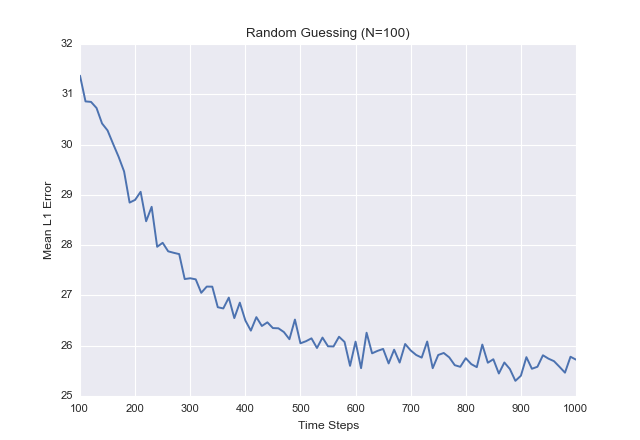
\includegraphics[width=0.5\textwidth]{figures/robustness/Random_Guessing21.png}%
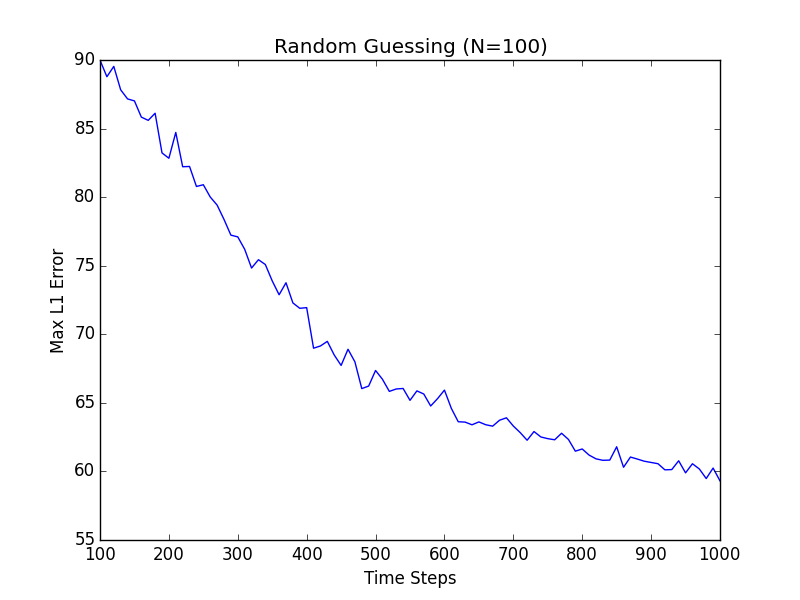
\includegraphics[width=0.5\textwidth] {figures/robustness/Random_Guessing22.png}%
}%
\caption{Mean and maximum $L_1$ error of Smarts Ratings when all $N$ players use a Random Guessing strategy. In Random Guessing, a player's Reported Guess is a random element from the domain of Smarts Ratings that is completely independent from the Actual Guess. These results establish baselines for subsequent simulations.}
\label{fig:RandomGuess}
\end{figure}

\subsubsection{Honest Play}

Honest players give Reported Guesses that are equivalent to their Actual Guesses. If all players are honest, Smarts Ratings quickly converge to Intelligences, as shown in Figure \ref{fig:HonestGuess}. Inducing honest play should be the foremost goal of LRS designers.

\begin{figure}[h]
\centerline{%
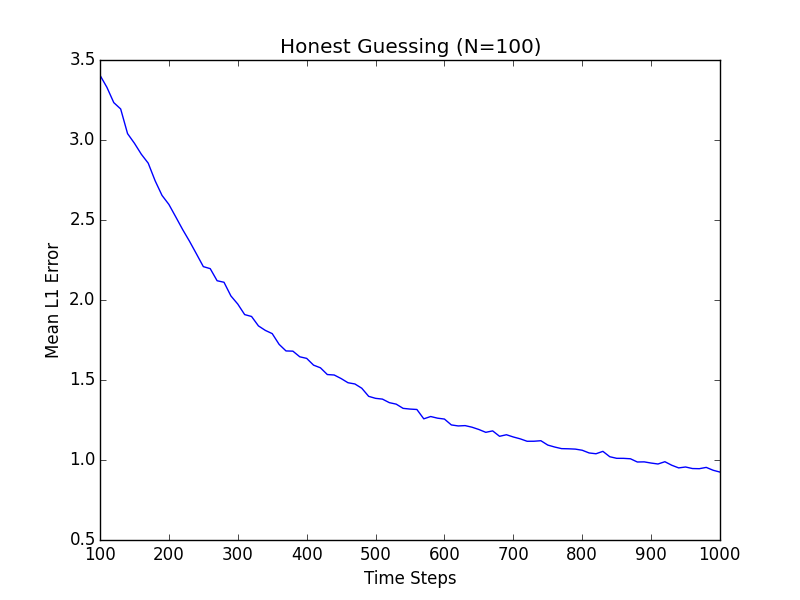
\includegraphics[width=0.5\textwidth]{figures/robustness/Honest_Guessing21.png}%
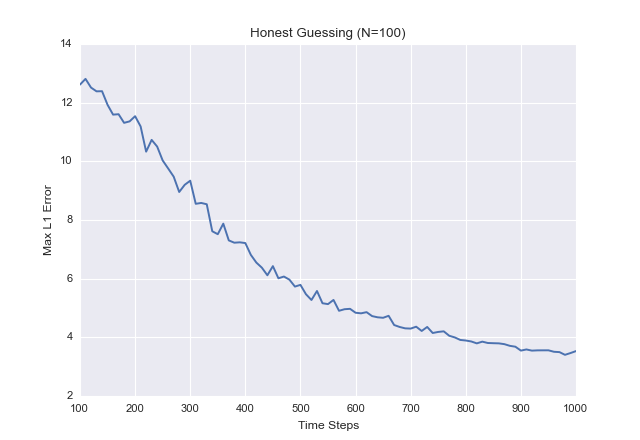
\includegraphics[width=0.5\textwidth] {figures/robustness/Honest_Guessing22.png}%
}%
\caption{Mean and maximum $L_1$ error of Smarts Ratings when all $N$ players Guess honestly. Honest play is defined by consistent equivalence between the player's Reported Guesses and Actual Guesses. Smarts Ratings quickly converge to intelligences if all players are honest.}
\label{fig:HonestGuess}
\end{figure}

\subsubsection{Single Priority Play}

If a player cares only about maximizing relative Smarts Ratings and neglects Luna Game outcomes, that player will likely give Reported Guesses of $0$ for all opponents. If all players use this Minimum Guessing strategy, Smarts Ratings will immediately collapse to $0$. More generally, the error introduced by Minimum Guessing depends linearly on the number of players using this strategy. Figure \ref{fig:MinimumGuess} confirms this result suggested by the theory. Mean $L_1$ error ranges from half the total range of Smarts Ratings to $0$.

\begin{figure}[H]
\centerline{%
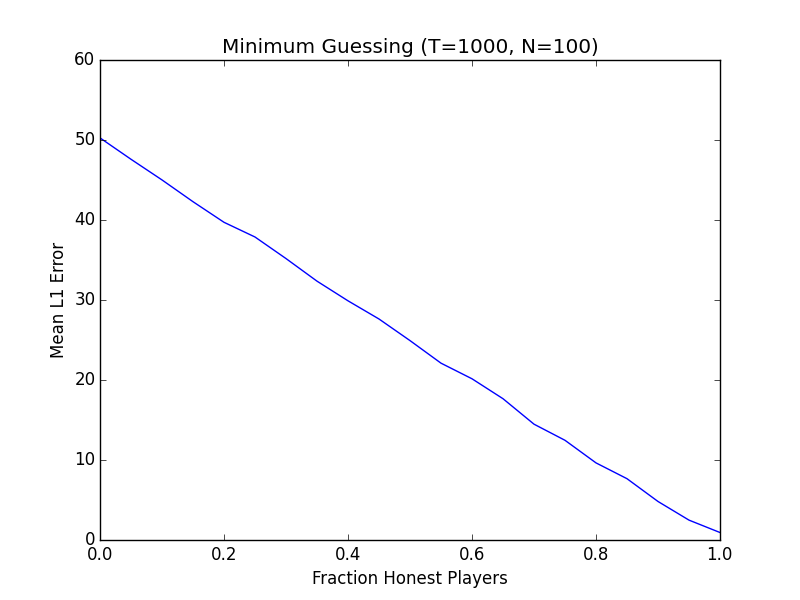
\includegraphics[width=0.5\textwidth]{figures/robustness/Minimum_Guessing31.png}%
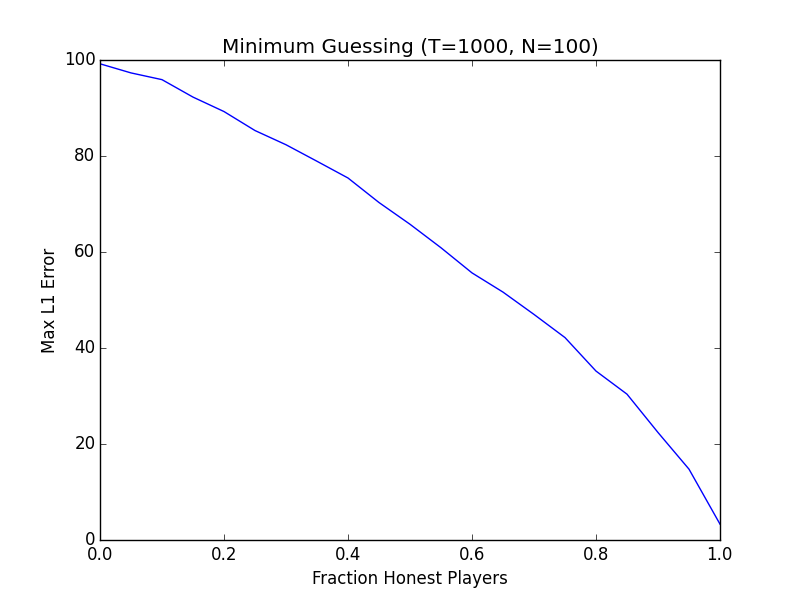
\includegraphics[width=0.5\textwidth] {figures/robustness/Minimum_Guessing32.png}%
}%
\caption{Mean and maximum $L_1$ error of Smarts Ratings when a fraction of the $N$ players use Minimum Guessing after $T$ time steps. In Minimum Guessing, a player always gives Reported Guesses of $0$. The error introduced by Minimum Guessing depends linearly on the number of players using the strategy.}
\label{fig:MinimumGuess}
\end{figure}

\subsubsection{Response Agnostic Play}

If the distribution of current Smarts Ratings is known at all times to all players, some players may try to take advantage of the distribution to formulate their Guesses. A naive approach is to give Reported Guesses equal to the current mean Smarts Rating. With all players using this approach, the distribution collapses and error explodes. In general, Figure \ref{fig:MeanGuess} shows that the error introduced by Mean Guessing depends linearly on the number of players using the strategy.

\begin{figure}[H]
\centerline{%
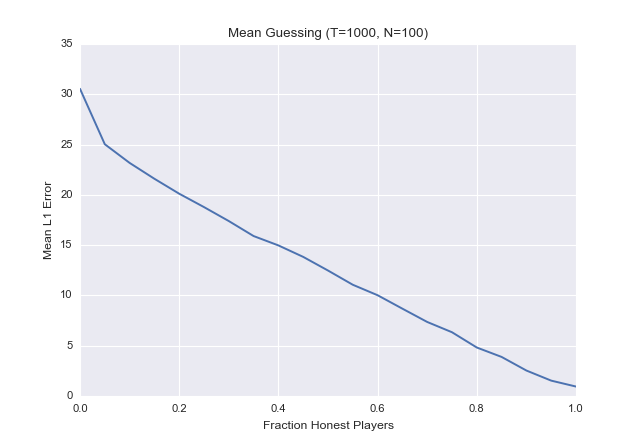
\includegraphics[width=0.5\textwidth]{figures/robustness/Mean_Guessing31.png}%
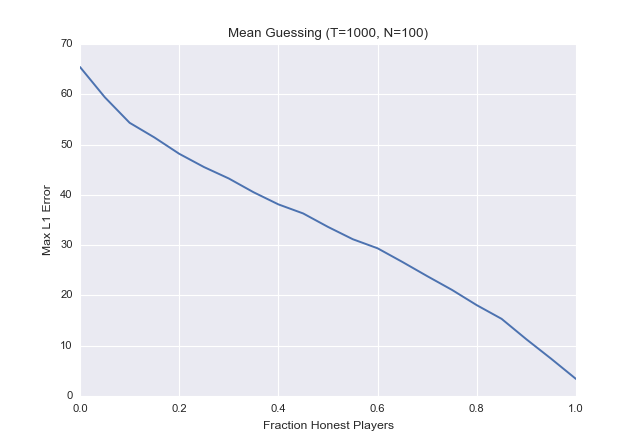
\includegraphics[width=0.5\textwidth] {figures/robustness/Mean_Guessing32.png}%
}%
\caption{Mean and maximum $L_1$ error of Smarts Ratings when a fraction of the $N$ players use Mean Guessing after $T$ time steps. In Mean Guessing, a player always gives Reported Guesses equal to the mean of all Smarts Ratings in the system. The error introduced by Mean Guessing depends linearly on the number of players using the strategy.}
\label{fig:MeanGuess}
\end{figure}

Another way that players may take advantage of a known distribution is via the Quantile Guessing strategy described above. The implementation of Quantile Guessing used for simulations uses the Empirical Cumulative Distribution Function with the sample composed of Actual Guesses of past opponents. A Reported Guess defaults to Actual Guesses if no Smarts Ratings have been determined, and for a player's first Luna Game. Ratings again collapse if all players use this strategy from the start, as shown in Figure \ref{fig:QuantileGuess}. 

\begin{figure}[H]
\centerline{%
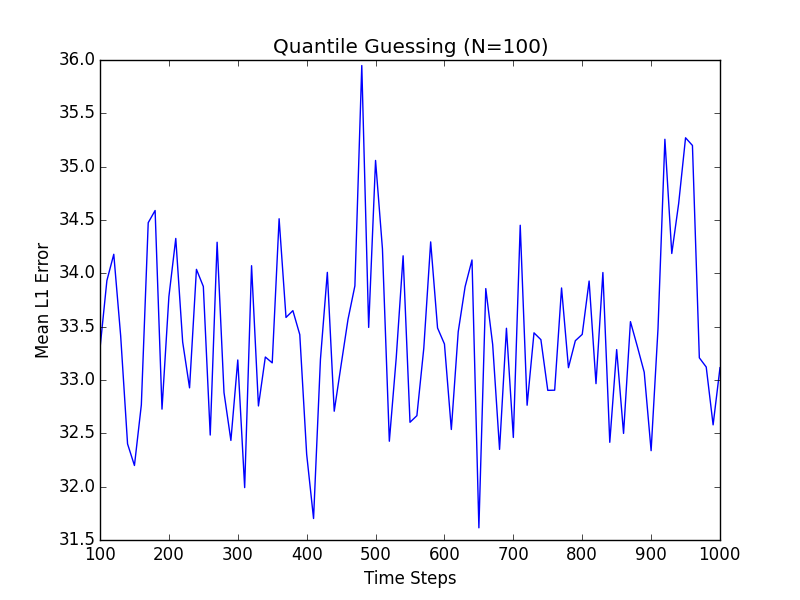
\includegraphics[width=0.5\textwidth]{figures/robustness/Quantile_Guessing21.png}%
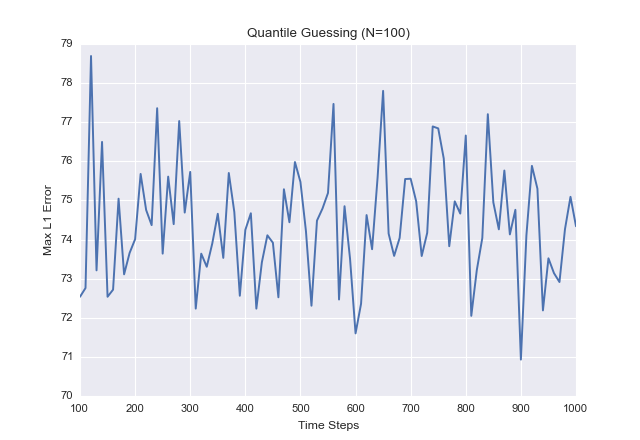
\includegraphics[width=0.5\textwidth] {figures/robustness/Quantile_Guessing22.png}%
}%
\caption{Mean and maximum $L_1$ error of Smarts Ratings when all $N$ players use Quantile Guessing. Quantile Guessing takes advantage of the distribution of all Smarts Ratings and a player's estimation of an opponent's rating percentile to formulate Reported Guesses. Due to the discrete nature of Smarts Ratings, Quantile Guessing causes Smarts Ratings to collapse to a constant, and the system cannot recover.}
\label{fig:QuantileGuess}
\end{figure}

If only a fraction of players use the strategy, the error depends linearly on the fraction, as was the case with Minimum and Mean Guessing. Figure \ref{fig:QuantileGuessFrac} confirms this result.

\begin{figure}[H]
\centerline{%
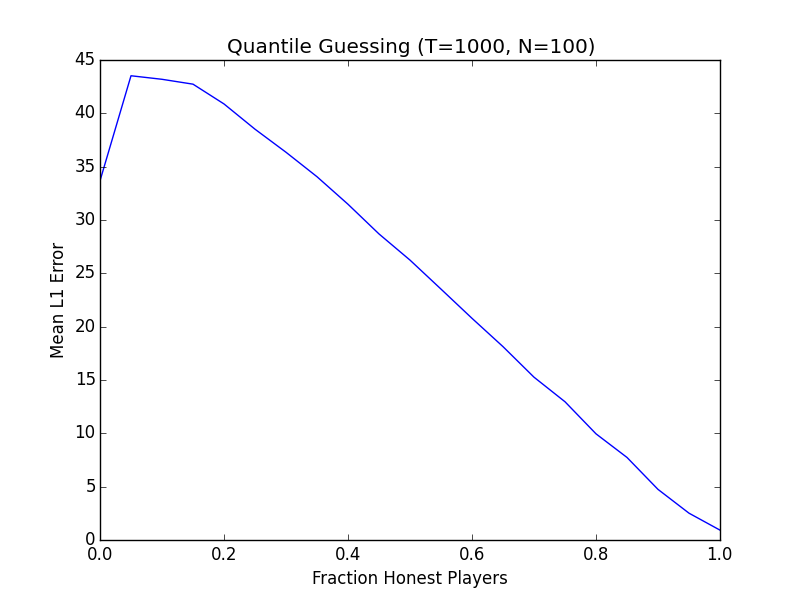
\includegraphics[width=0.5\textwidth]{figures/robustness/Quantile_Guessing31.png}%
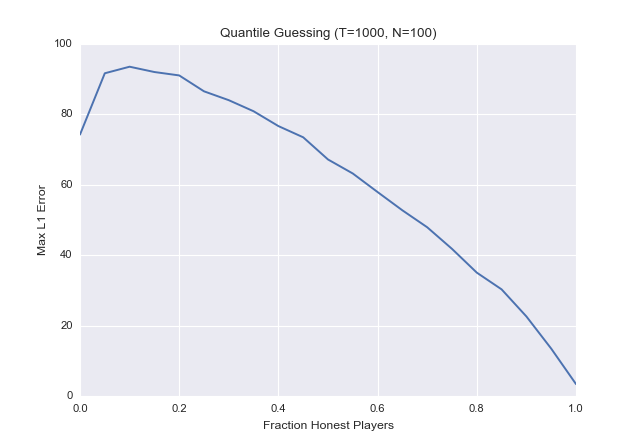
\includegraphics[width=0.5\textwidth] {figures/robustness/Quantile_Guessing32.png}%
}%
\caption{Mean and maximum $L_1$ error of Smarts Ratings when a fraction of $N$ players use Quantile Guessing after $T$ time steps. Quantile Guessing takes advantage of the distribution of all Smarts Ratings and a player's estimation of an opponent's rating percentile to formulate Reported Guesses. The error introduced by Quantile Guessing depends linearly on the number of players using the strategy.}
\label{fig:QuantileGuessFrac}
\end{figure}

What if the distribution is revealed once a certain number of games have been played? Perhaps the collapsing to a constant problem will be avoided? To test this hypothesis, the simulation in Figure \ref{fig:QuantileGuessDelay} introduces players that play with honest guessing for a variable number of time steps, and then play with Quantile Guessing for $500$ time steps. The delay in introducing Quantile Guessing does indeed improve the $L_1$ error within the time frame tested, though significant error remains after $500$ time steps for all tested delays. 

\begin{figure}[H]
\centerline{%
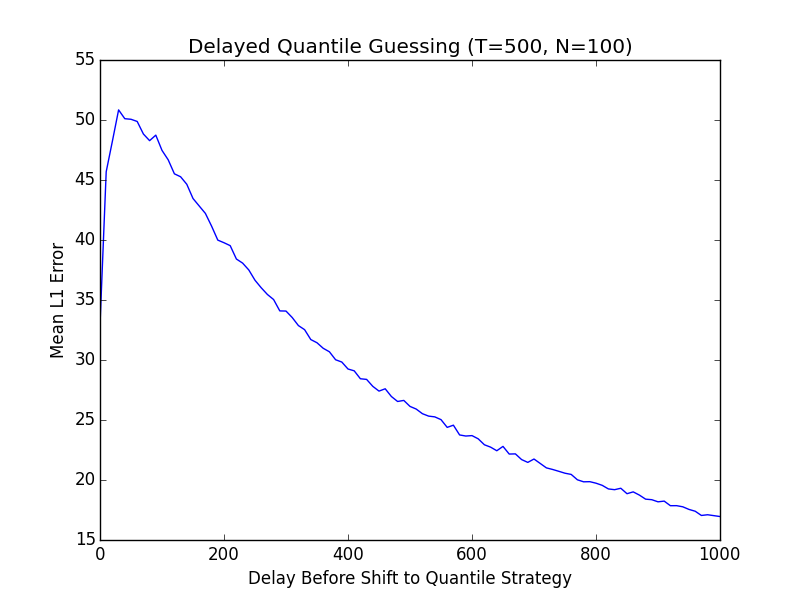
\includegraphics[width=0.5\textwidth]{figures/robustness/Delayed_Quantile_Guessing41.png}%
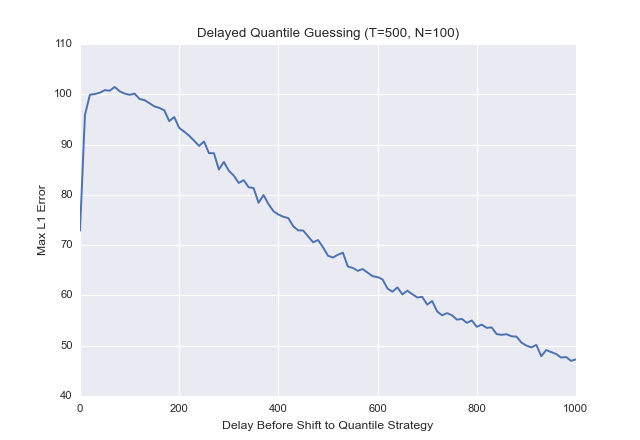
\includegraphics[width=0.5\textwidth] {figures/robustness/Delayed_Quantile_Guessing42.png}%
}%
\caption{Mean and maximum $L_1$ error of Smarts Ratings when $N$ players give honest guesses for some number of delay time steps, and then shift to the Quantile Guessing strategy for 500 additional time steps. The shift delay is negatively correlated with Quantile Guessing, suggesting that the negative impact of the strategy decreases if it is introduced after LRS has already stabilized.}
\label{fig:QuantileGuessDelay}
\end{figure}

\subsection{Combined Strategies}

In a real instantiation of LRS, it is unlikely that any single strategy will be adopted by all players. Thus the extreme results portrayed above are not of urgent concern. More likely is a situation where a small fraction of players adopt each of the strategies above. For the purpose of simulation, I assume that some fraction of players will play honestly, and the remaining players will be evenly divided among the strategies described above: Random Guessing, Minimum Guessing, Mean Guessing, and Quantile Guessing. Figure \ref{fig:Combined} shows that the relationship between error and honest player proportion is linear, as might be expected given the previous simulations. Roughly, for every additional $10$\% of players that forgo honest guessing in favor of one of the other strategies, the mean $L_1$ error increases by $3.5$.

\begin{figure}[H]
\centerline{%
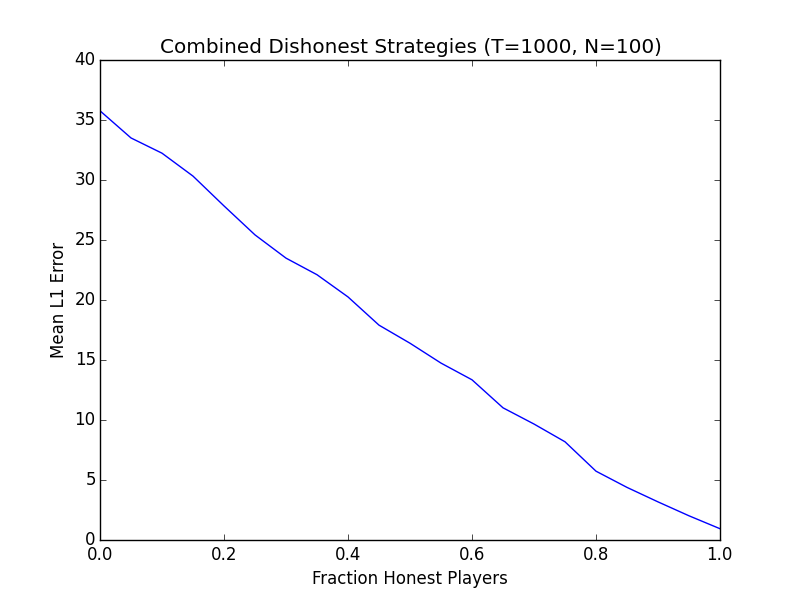
\includegraphics[width=0.5\textwidth]{figures/robustness/Combined_Dishonest_Strategies31.png}
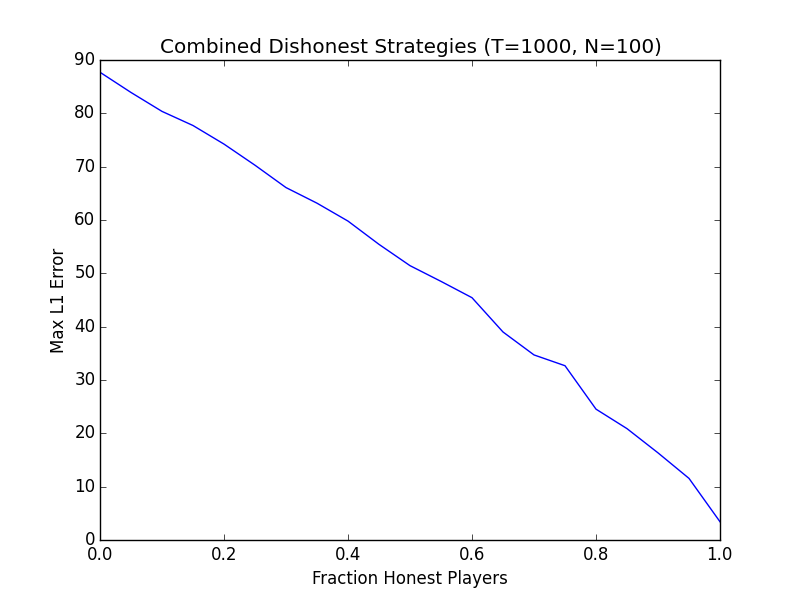
\includegraphics[width=0.5\textwidth] {figures/robustness/Combined_Dishonest_Strategies32.png}%
}%
\caption{Mean and maximum $L_1$ error of Smarts Ratings when some fraction of $N$ players give honest guesses, and the remaining players are split evenly among Random Guessing, Minimum Guessing, Mean Guessing, and Quantile Guessing strategies. The relationship between error and honest player proportion is linear.}
\label{fig:Combined}
\end{figure}
\section{Implications for LRS Design}

The theoretical and simulation results discussed in this chapter provide a cautionary tale for LRS designers. The system should be successful if all players practice honest play, but other strategies, such as Random Guessing, Minimum Guessing, Mean Guessing, and Quantile Guessing, threaten to undermine the validity of Smarts Ratings. Fortunately, these strategies can be grouped into two categories: strategies that are unlikely, and strategies that can be prevented. 

Random Guessing and Minimum Guessing belong in the unlikely strategy group. Random Guessing would be a bizarre long-term choice; the strategy gives a player no advantage in either Smarts Rating or Luna Game outcomes. Minimum Guessing is also unlikely for the player who realizes the personal benefit in terms of relative Smarts Ratings is very small. Minimum Guessing can also claim membership to the preventable strategy group; players practicing this strategy can be quickly identified by the system and banned for violating the spirit of play. Since they rely on the distribution of Smarts Ratings, Mean Guessing and Quantile Guessing are also easily avoidable; the distribution can simply be withheld from players. The distribution may also be withheld initially and introduced once the system has evolved and stabilized. This delay would improve Quantile Guessing for players, and these later players would introduce less error to Smarts Ratings by using the strategy.

If the Smarts Rating distribution is withheld from players, designers must choose another method for describing the ratings, or else the players will have no basis to form their first Guesses. This chapter has discussed several avenues that should be avoided: fixed initializations of Smarts Ratings; a first-time ``quiz'' to initialize Smarts Ratings; or communicating only the average Smarts Rating. One option is to provide a vague disclaimer, such as ``Smarts Ratings are positive real numbers that typically range between $0$ and $100$.'' A more concrete alternative would be to ask players, ``On a scale from $0$ to $100$, how smart is your opponent?'' Of course, providing any numbers in the instructions encourages machine players to adopt Means Guessing or a similar naive strategy early on. Initializing these early Smarts Ratings is ultimately a chicken-or-egg problem that can only be resolved in practice by well-meaning human players.

The results in this chapter underscore the importance of good faith among players of the Luna Game. For researchers hoping to use LRS as a test of AI, the integrity of the system is essential if their own results are to be meaningful. Honest play is in the best interest of these players. Casual human players should also understand that dishonest strategies in mass can threaten both the validity and the distribution of Smarts Ratings, rendering LRS neither informative nor fun for players. The spirit of the Game should be made as clear to players as the limited attention span of Internet users permits. As with any test of human intelligence, LRS ultimately requires judges and subjects to play along.

%\chapter{Conclusion}
\label{conclusion}

Lorem ipsum dolor sit amet, consectetuer adipiscing elit. Morbi commodo, ipsum sed pharetra gravida, orci magna rhoncus neque, id pulvinar odio lorem non turpis. Nullam sit amet enim. Suspendisse id velit vitae ligula volutpat condimentum. Aliquam erat volutpat. Sed quis velit. Nulla facilisi. Nulla libero. Vivamus pharetra posuere sapien. Nam consectetuer. Sed aliquam, nunc eget euismod ullamcorper, lectus nunc ullamcorper orci, fermentum bibendum enim nibh eget ipsum. Donec porttitor ligula eu dolor. Maecenas vitae nulla consequat libero cursus venenatis. Nam magna enim, accumsan eu, blandit sed, blandit a, eros.

Quisque facilisis erat a dui. Nam malesuada ornare dolor. Cras gravida, diam sit amet rhoncus ornare, erat elit consectetuer erat, id egestas pede nibh eget odio. Proin tincidunt, velit vel porta elementum, magna diam molestie sapien, non aliquet massa pede eu diam. Aliquam iaculis. Fusce et ipsum et nulla tristique facilisis. Donec eget sem sit amet ligula viverra gravida. Etiam vehicula urna vel turpis. Suspendisse sagittis ante a urna. Morbi a est quis orci consequat rutrum. Nullam egestas feugiat felis. Integer adipiscing semper ligula. Nunc molestie, nisl sit amet cursus convallis, sapien lectus pretium metus, vitae pretium enim wisi id lectus. Donec vestibulum. Etiam vel nibh. Nulla facilisi. Mauris pharetra. Donec augue. Fusce ultrices, neque id dignissim ultrices, tellus mauris dictum elit, vel lacinia enim metus eu nunc.

Pellentesque habitant morbi tristique senectus et netus et malesuada fames ac turpis egestas. Vestibulum tortor quam, feugiat vitae, ultricies eget, tempor sit amet, ante. Donec eu libero sit amet quam egestas semper. Aenean ultricies mi vitae est. Mauris placerat eleifend leo. Quisque sit amet est et sapien ullamcorper pharetra. Vestibulum erat wisi, condimentum sed, commodo vitae, ornare sit amet, wisi. Aenean fermentum, elit eget tincidunt condimentum, eros ipsum rutrum orci, sagittis tempus lacus enim ac dui. Donec non enim in turpis pulvinar facilisis. Ut felis.

Cras sed ante. Phasellus in massa. Curabitur dolor eros, gravida et, hendrerit ac, cursus non, massa. Aliquam lorem. In hac habitasse platea dictumst. Cras eu mauris. Quisque lacus. Donec ipsum. Nullam vitae sem at nunc pharetra ultricies. Vivamus elit eros, ullamcorper a, adipiscing sit amet, porttitor ut, nibh. Maecenas adipiscing mollis massa. Nunc ut dui eget nulla venenatis aliquet. Sed luctus posuere justo. Cras vehicula varius turpis. Vivamus eros metus, tristique sit amet, molestie dignissim, malesuada et, urna.

Cras dictum. Maecenas ut turpis. In vitae erat ac orci dignissim eleifend. Nunc quis justo. Sed vel ipsum in purus tincidunt pharetra. Sed pulvinar, felis id consectetuer malesuada, enim nisl mattis elit, a facilisis tortor nibh quis leo. Sed augue lacus, pretium vitae, molestie eget, rhoncus quis, elit. Donec in augue. Fusce orci wisi, ornare id, mollis vel, lacinia vel, massa.

Lorem ipsum dolor sit amet, consectetuer adipiscing elit. Morbi commodo, ipsum sed pharetra gravida, orci magna rhoncus neque, id pulvinar odio lorem non turpis. Nullam sit amet enim. Suspendisse id velit vitae ligula volutpat condimentum. Aliquam erat volutpat. Sed quis velit. Nulla facilisi. Nulla libero. Vivamus pharetra posuere sapien. Nam consectetuer. Sed aliquam, nunc eget euismod ullamcorper, lectus nunc ullamcorper orci, fermentum bibendum enim nibh eget ipsum. Donec porttitor ligula eu dolor. Maecenas vitae nulla consequat libero cursus venenatis. Nam magna enim, accumsan eu, blandit sed, blandit a, eros.

Quisque facilisis erat a dui. Nam malesuada ornare dolor. Cras gravida, diam sit amet rhoncus ornare, erat elit consectetuer erat, id egestas pede nibh eget odio. Proin tincidunt, velit vel porta elementum, magna diam molestie sapien, non aliquet massa pede eu diam. Aliquam iaculis. Fusce et ipsum et nulla tristique facilisis. Donec eget sem sit amet ligula viverra gravida. Etiam vehicula urna vel turpis. Suspendisse sagittis ante a urna. Morbi a est quis orci consequat rutrum. Nullam egestas feugiat felis. Integer adipiscing semper ligula. Nunc molestie, nisl sit amet cursus convallis, sapien lectus pretium metus, vitae pretium enim wisi id lectus. Donec vestibulum. Etiam vel nibh. Nulla facilisi. Mauris pharetra. Donec augue. Fusce ultrices, neque id dignissim ultrices, tellus mauris dictum elit, vel lacinia enim metus eu nunc.

%\begin{appendices}
%    \chapter{Some extra stuff}
\label{AppendixA}

Lorem ipsum dolor sit amet, consectetuer adipiscing elit. Morbi commodo, ipsum sed pharetra gravida, orci magna rhoncus neque, id pulvinar odio lorem non turpis. Nullam sit amet enim. Suspendisse id velit vitae ligula volutpat condimentum. Aliquam erat volutpat. Sed quis velit. Nulla facilisi. Nulla libero. Vivamus pharetra posuere sapien. Nam consectetuer. Sed aliquam, nunc eget euismod ullamcorper, lectus nunc ullamcorper orci, fermentum bibendum enim nibh eget ipsum. Donec porttitor ligula eu dolor. Maecenas vitae nulla consequat libero cursus venenatis. Nam magna enim, accumsan eu, blandit sed, blandit a, eros.

Quisque facilisis erat a dui. Nam malesuada ornare dolor. Cras gravida, diam sit amet rhoncus ornare, erat elit consectetuer erat, id egestas pede nibh eget odio. Proin tincidunt, velit vel porta elementum, magna diam molestie sapien, non aliquet massa pede eu diam. Aliquam iaculis. Fusce et ipsum et nulla tristique facilisis. Donec eget sem sit amet ligula viverra gravida. Etiam vehicula urna vel turpis. Suspendisse sagittis ante a urna. Morbi a est quis orci consequat rutrum. Nullam egestas feugiat felis. Integer adipiscing semper ligula. Nunc molestie, nisl sit amet cursus convallis, sapien lectus pretium metus, vitae pretium enim wisi id lectus. Donec vestibulum. Etiam vel nibh. Nulla facilisi. Mauris pharetra. Donec augue. Fusce ultrices, neque id dignissim ultrices, tellus mauris dictum elit, vel lacinia enim metus eu nunc.

Pellentesque habitant morbi tristique senectus et netus et malesuada fames ac turpis egestas. Vestibulum tortor quam, feugiat vitae, ultricies eget, tempor sit amet, ante. Donec eu libero sit amet quam egestas semper. Aenean ultricies mi vitae est. Mauris placerat eleifend leo. Quisque sit amet est et sapien ullamcorper pharetra. Vestibulum erat wisi, condimentum sed, commodo vitae, ornare sit amet, wisi. Aenean fermentum, elit eget tincidunt condimentum, eros ipsum rutrum orci, sagittis tempus lacus enim ac dui. Donec non enim in turpis pulvinar facilisis. Ut felis.

Cras sed ante. Phasellus in massa. Curabitur dolor eros, gravida et, hendrerit ac, cursus non, massa. Aliquam lorem. In hac habitasse platea dictumst. Cras eu mauris. Quisque lacus. Donec ipsum. Nullam vitae sem at nunc pharetra ultricies. Vivamus elit eros, ullamcorper a, adipiscing sit amet, porttitor ut, nibh. Maecenas adipiscing mollis massa. Nunc ut dui eget nulla venenatis aliquet. Sed luctus posuere justo. Cras vehicula varius turpis. Vivamus eros metus, tristique sit amet, molestie dignissim, malesuada et, urna.

Cras dictum. Maecenas ut turpis. In vitae erat ac orci dignissim eleifend. Nunc quis justo. Sed vel ipsum in purus tincidunt pharetra. Sed pulvinar, felis id consectetuer malesuada, enim nisl mattis elit, a facilisis tortor nibh quis leo. Sed augue lacus, pretium vitae, molestie eget, rhoncus quis, elit. Donec in augue. Fusce orci wisi, ornare id, mollis vel, lacinia vel, massa.

Lorem ipsum dolor sit amet, consectetuer adipiscing elit. Morbi commodo, ipsum sed pharetra gravida, orci magna rhoncus neque, id pulvinar odio lorem non turpis. Nullam sit amet enim. Suspendisse id velit vitae ligula volutpat condimentum. Aliquam erat volutpat. Sed quis velit. Nulla facilisi. Nulla libero. Vivamus pharetra posuere sapien. Nam consectetuer. Sed aliquam, nunc eget euismod ullamcorper, lectus nunc ullamcorper orci, fermentum bibendum enim nibh eget ipsum. Donec porttitor ligula eu dolor. Maecenas vitae nulla consequat libero cursus venenatis. Nam magna enim, accumsan eu, blandit sed, blandit a, eros.

Quisque facilisis erat a dui. Nam malesuada ornare dolor. Cras gravida, diam sit amet rhoncus ornare, erat elit consectetuer erat, id egestas pede nibh eget odio. Proin tincidunt, velit vel porta elementum, magna diam molestie sapien, non aliquet massa pede eu diam. Aliquam iaculis. Fusce et ipsum et nulla tristique facilisis. Donec eget sem sit amet ligula viverra gravida. Etiam vehicula urna vel turpis. Suspendisse sagittis ante a urna. Morbi a est quis orci consequat rutrum. Nullam egestas feugiat felis. Integer adipiscing semper ligula. Nunc molestie, nisl sit amet cursus convallis, sapien lectus pretium metus, vitae pretium enim wisi id lectus. Donec vestibulum. Etiam vel nibh. Nulla facilisi. Mauris pharetra. Donec augue. Fusce ultrices, neque id dignissim ultrices, tellus mauris dictum elit, vel lacinia enim metus eu nunc.

%\end{appendices}
%
%\setstretch{1.2}
%
% the back matter
\clearpage
\bibliography{VVT_Thesis_References}
\addcontentsline{toc}{chapter}{References}
\bibliographystyle{apalike2}

%\newpage

% If you do want an image in the colophon:
\begin{figure}
  \vspace{20pt}
  \centering
  \hspace*{-32pt}
  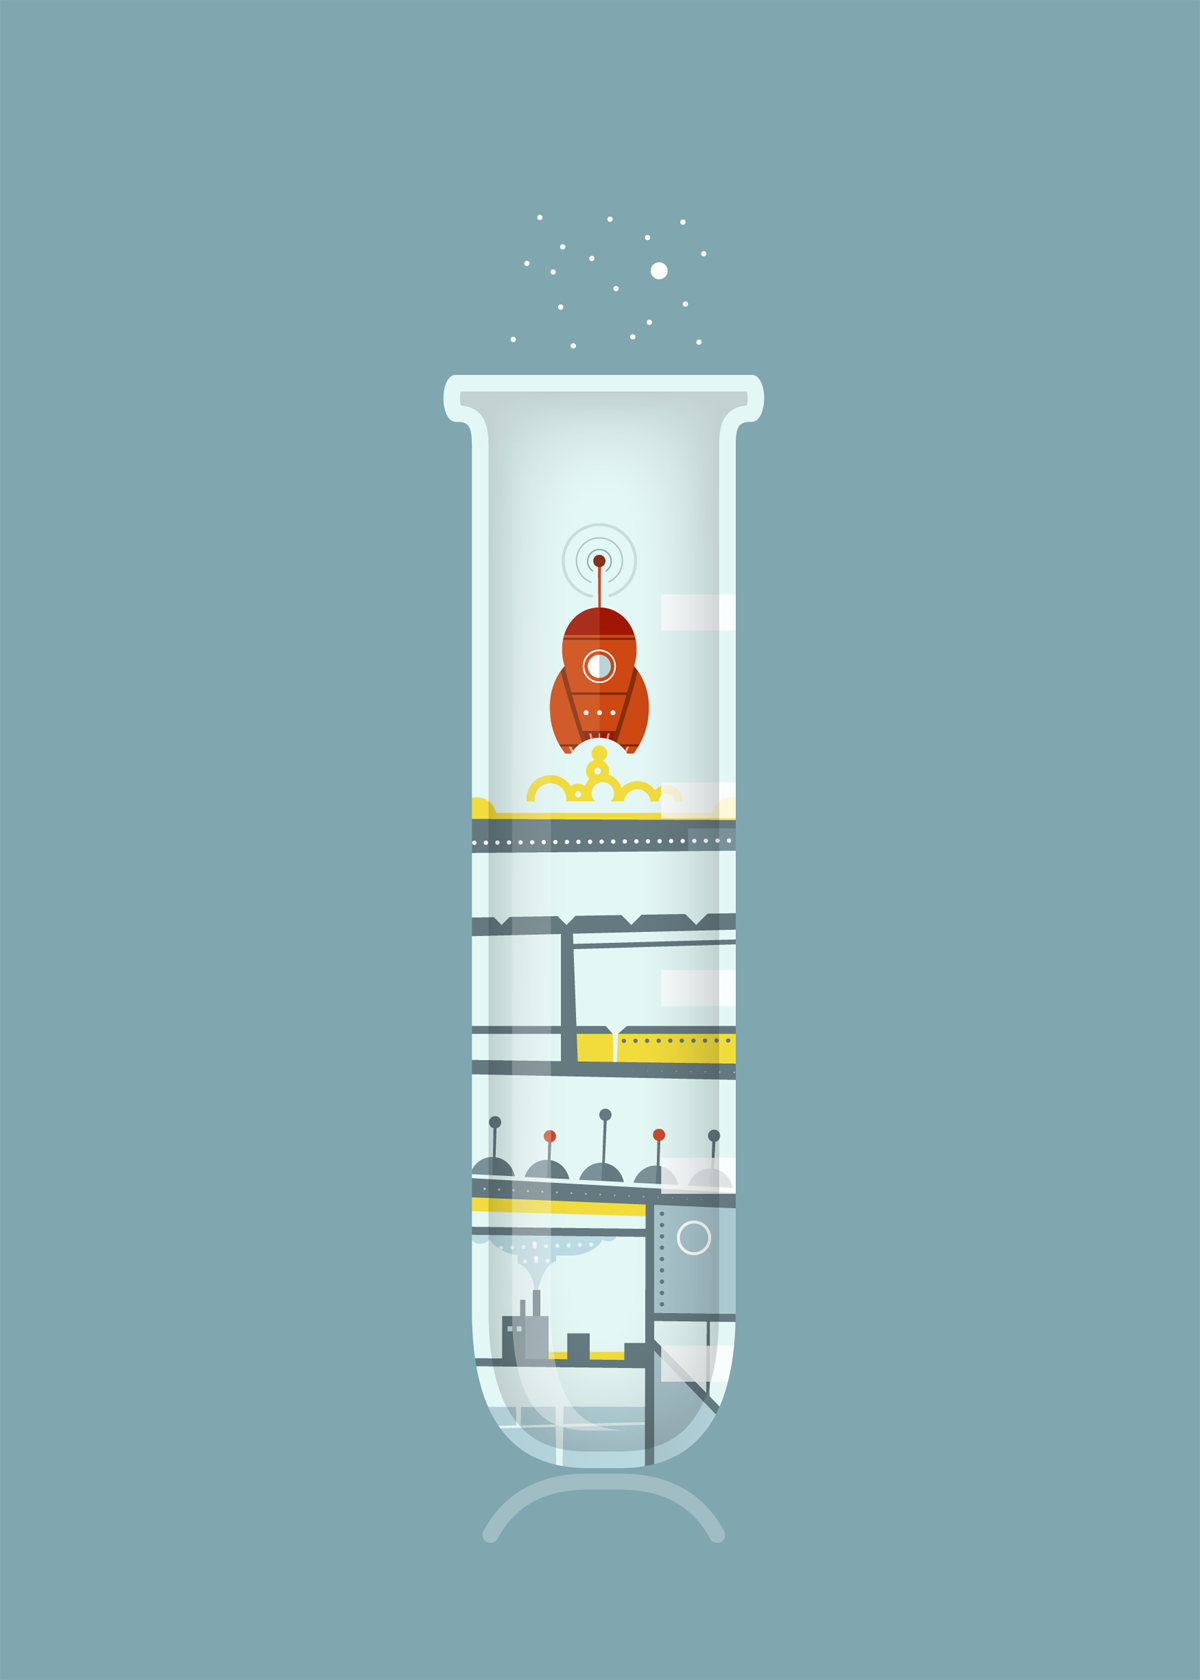
\includegraphics[width=0.42\textwidth]{endmatter/colophon.png}
\end{figure}

% If you don't want an image in the colophon:
% \vspace*{200pt}

\begin{center}
\parbox{200pt}{\lettrine[lines=3,slope=-2pt,nindent=-4pt]{\textcolor{SchoolColor}{T}}{his thesis was typeset} using \LaTeX, originally developed by Leslie Lamport and based on Donald Knuth's \TeX. The body text is set in 11 point Egenolff-Berner Garamond, a revival of Claude Garamont's humanist typeface. The above illustration, \textit{Science Experiment 02}, was created by Ben Schlitter and released under \href{http://creativecommons.org/licenses/by-nc-nd/3.0/}{\textsc{cc by-nc-nd 3.0}}. A template that can be used to format a PhD dissertation with this look \textit{\&} feel has been released under the permissive \textsc{agpl} license, and can be found online at \href{https://github.com/asm-products/Dissertate}{github.com/asm-products/Dissertate} or from its lead author, Jordan Suchow, at \href{mailto:suchow@post.harvard.edu}{suchow@post.harvard.edu}.}
\end{center}


\end{document}
